% Options for packages loaded elsewhere
\PassOptionsToPackage{unicode}{hyperref}
\PassOptionsToPackage{hyphens}{url}
\PassOptionsToPackage{dvipsnames,svgnames,x11names}{xcolor}
%
\documentclass[
  12pt,
]{article}

\usepackage{amsmath,amssymb}
\usepackage{setspace}
\usepackage{iftex}
\ifPDFTeX
  \usepackage[T1]{fontenc}
  \usepackage[utf8]{inputenc}
  \usepackage{textcomp} % provide euro and other symbols
\else % if luatex or xetex
  \usepackage{unicode-math}
  \defaultfontfeatures{Scale=MatchLowercase}
  \defaultfontfeatures[\rmfamily]{Ligatures=TeX,Scale=1}
\fi
\usepackage{lmodern}
\ifPDFTeX\else  
    % xetex/luatex font selection
  \setmainfont[]{Times New Roman}
\fi
% Use upquote if available, for straight quotes in verbatim environments
\IfFileExists{upquote.sty}{\usepackage{upquote}}{}
\IfFileExists{microtype.sty}{% use microtype if available
  \usepackage[]{microtype}
  \UseMicrotypeSet[protrusion]{basicmath} % disable protrusion for tt fonts
}{}
\makeatletter
\@ifundefined{KOMAClassName}{% if non-KOMA class
  \IfFileExists{parskip.sty}{%
    \usepackage{parskip}
  }{% else
    \setlength{\parindent}{0pt}
    \setlength{\parskip}{6pt plus 2pt minus 1pt}}
}{% if KOMA class
  \KOMAoptions{parskip=half}}
\makeatother
\usepackage{xcolor}
\usepackage[margin=2cm]{geometry}
\setlength{\emergencystretch}{3em} % prevent overfull lines
\setcounter{secnumdepth}{5}
% Make \paragraph and \subparagraph free-standing
\ifx\paragraph\undefined\else
  \let\oldparagraph\paragraph
  \renewcommand{\paragraph}[1]{\oldparagraph{#1}\mbox{}}
\fi
\ifx\subparagraph\undefined\else
  \let\oldsubparagraph\subparagraph
  \renewcommand{\subparagraph}[1]{\oldsubparagraph{#1}\mbox{}}
\fi


\providecommand{\tightlist}{%
  \setlength{\itemsep}{0pt}\setlength{\parskip}{0pt}}\usepackage{longtable,booktabs,array}
\usepackage{calc} % for calculating minipage widths
% Correct order of tables after \paragraph or \subparagraph
\usepackage{etoolbox}
\makeatletter
\patchcmd\longtable{\par}{\if@noskipsec\mbox{}\fi\par}{}{}
\makeatother
% Allow footnotes in longtable head/foot
\IfFileExists{footnotehyper.sty}{\usepackage{footnotehyper}}{\usepackage{footnote}}
\makesavenoteenv{longtable}
\usepackage{graphicx}
\makeatletter
\def\maxwidth{\ifdim\Gin@nat@width>\linewidth\linewidth\else\Gin@nat@width\fi}
\def\maxheight{\ifdim\Gin@nat@height>\textheight\textheight\else\Gin@nat@height\fi}
\makeatother
% Scale images if necessary, so that they will not overflow the page
% margins by default, and it is still possible to overwrite the defaults
% using explicit options in \includegraphics[width, height, ...]{}
\setkeys{Gin}{width=\maxwidth,height=\maxheight,keepaspectratio}
% Set default figure placement to htbp
\makeatletter
\def\fps@figure{htbp}
\makeatother
% definitions for citeproc citations
\NewDocumentCommand\citeproctext{}{}
\NewDocumentCommand\citeproc{mm}{%
  \begingroup\def\citeproctext{#2}\cite{#1}\endgroup}
\makeatletter
 % allow citations to break across lines
 \let\@cite@ofmt\@firstofone
 % avoid brackets around text for \cite:
 \def\@biblabel#1{}
 \def\@cite#1#2{{#1\if@tempswa , #2\fi}}
\makeatother
\newlength{\cslhangindent}
\setlength{\cslhangindent}{1.5em}
\newlength{\csllabelwidth}
\setlength{\csllabelwidth}{3em}
\newenvironment{CSLReferences}[2] % #1 hanging-indent, #2 entry-spacing
 {\begin{list}{}{%
  \setlength{\itemindent}{0pt}
  \setlength{\leftmargin}{0pt}
  \setlength{\parsep}{0pt}
  % turn on hanging indent if param 1 is 1
  \ifodd #1
   \setlength{\leftmargin}{\cslhangindent}
   \setlength{\itemindent}{-1\cslhangindent}
  \fi
  % set entry spacing
  \setlength{\itemsep}{#2\baselineskip}}}
 {\end{list}}
\usepackage{calc}
\newcommand{\CSLBlock}[1]{\hfill\break\parbox[t]{\linewidth}{\strut\ignorespaces#1\strut}}
\newcommand{\CSLLeftMargin}[1]{\parbox[t]{\csllabelwidth}{\strut#1\strut}}
\newcommand{\CSLRightInline}[1]{\parbox[t]{\linewidth - \csllabelwidth}{\strut#1\strut}}
\newcommand{\CSLIndent}[1]{\hspace{\cslhangindent}#1}

\usepackage{booktabs}
\usepackage{longtable}
\usepackage{array}
\usepackage{multirow}
\usepackage{wrapfig}
\usepackage{float}
\usepackage{colortbl}
\usepackage{pdflscape}
\usepackage{tabu}
\usepackage{threeparttable}
\usepackage{threeparttablex}
\usepackage[normalem]{ulem}
\usepackage{makecell}
\usepackage{xcolor}
\usepackage[noblocks]{authblk}
\renewcommand*{\Authsep}{, }
\renewcommand*{\Authand}{, }
\renewcommand*{\Authands}{, }
\renewcommand\Affilfont{\small}
\makeatletter
\@ifpackageloaded{caption}{}{\usepackage{caption}}
\AtBeginDocument{%
\ifdefined\contentsname
  \renewcommand*\contentsname{Table of contents}
\else
  \newcommand\contentsname{Table of contents}
\fi
\ifdefined\listfigurename
  \renewcommand*\listfigurename{List of Figures}
\else
  \newcommand\listfigurename{List of Figures}
\fi
\ifdefined\listtablename
  \renewcommand*\listtablename{List of Tables}
\else
  \newcommand\listtablename{List of Tables}
\fi
\ifdefined\figurename
  \renewcommand*\figurename{Figure}
\else
  \newcommand\figurename{Figure}
\fi
\ifdefined\tablename
  \renewcommand*\tablename{Table}
\else
  \newcommand\tablename{Table}
\fi
}
\@ifpackageloaded{float}{}{\usepackage{float}}
\floatstyle{ruled}
\@ifundefined{c@chapter}{\newfloat{codelisting}{h}{lop}}{\newfloat{codelisting}{h}{lop}[chapter]}
\floatname{codelisting}{Listing}
\newcommand*\listoflistings{\listof{codelisting}{List of Listings}}
\makeatother
\makeatletter
\makeatother
\makeatletter
\@ifpackageloaded{caption}{}{\usepackage{caption}}
\@ifpackageloaded{subcaption}{}{\usepackage{subcaption}}
\makeatother
\ifLuaTeX
  \usepackage{selnolig}  % disable illegal ligatures
\fi
\usepackage{bookmark}

\IfFileExists{xurl.sty}{\usepackage{xurl}}{} % add URL line breaks if available
\urlstyle{same} % disable monospaced font for URLs
\hypersetup{
  pdftitle={Perceptions of Inequality and Meritocracy: Their Interplay in Shaping Preferences for Market Justice in Chile (2016-2023)},
  pdfauthor={Equipo EDUMER},
  colorlinks=true,
  linkcolor={blue},
  filecolor={Maroon},
  citecolor={Blue},
  urlcolor={Blue},
  pdfcreator={LaTeX via pandoc}}

\title{Perceptions of Inequality and Meritocracy: Their Interplay in
Shaping Preferences for Market Justice in Chile (2016-2023)}


  \author{Juan Carlos Castillo}
            \affil{%
                  Departamento de Sociología, Universidad de Chile
              }
          \affil{%
                  Centro de estudios del conflicto y cohesión social
                  (COES)
              }
          \affil{%
                  Núcleo milenio de desigualdades y oportunidades
                  digitales (NUDOS)
              }
        \author{Andreas Laffert}
            \affil{%
                  Instituto de Sociología, Pontificia Universidad
                  Católica de Chile
              }
        \author{Kevin Carrasco}
            \affil{%
                  Centro de estudios del conflicto y cohesión social
                  (COES)
              }
        \author{Julio Iturra}
            \affil{%
                  International Graduate School of Social Sciencies
                  (BIGSSS), University of Bremen, Germany
              }
      
\date{}
\begin{document}
\maketitle
\begin{abstract}
This study investigates the relationship between perceptions of economic
inequality, meritocratic beliefs, and preferences for market justice in
Chile between 2016 and 2023. Using six waves of panel data from the
Chilean Longitudinal Social Survey - ELSOC (\(N_{observations}\) =
8,643; \(N_{individuals}\) = 1,687), the analysis examines how
subjective assessments of inequality shape attitudes toward the role of
merit in access to key social services such as healthcare, education,
and pensions. Results indicate that rising perceptions of inequality are
associated with greater support for redistributive policies; however,
individuals with strong meritocratic convictions are more likely to
legitimize existing disparities. The study also considers the influence
of major social movements during this period, which appear to have
reshaped public discourse and perceptions of fairness. These findings
contribute to a deeper understanding of how beliefs about justice and
equity evolve in contexts marked by persistent inequality and entrenched
market-oriented frameworks. \newline \textbf{Keywords}: Economic
inequality, meritocracy, market justice, Chile, public preferences,
inequality perception
\end{abstract}

\setstretch{1.15}
\section{Introduction}\label{introduction}

Since 1980, economic inequality and wealth concentration have
dramatically increased worldwide, becoming one of the main challenges
for the social sciences. Globally, in 2021, less than 50\% of the world
population owned only 2\% of the wealth, while the richest 10\%
concentrated 76\%, and the wealthiest 1\% captured nearly 38\% of total
assets (\citeproc{ref-chancel_world_2022}{Chancel et al., 2022}). This
context of economic disparity has sparked renewed interest in studying
not only the objective aspects of inequality, such as income and access
to resources, but also its subjective dimensions, including perceptions,
beliefs, and associated attitudes
(\citeproc{ref-janmaat_subjective_2013}{Janmaat, 2013}). This has led,
among other reasons, to widespread concern in the social sciences about
the political delegitimization that economic inequality can produce
(\citeproc{ref-castillo_perception_2022}{Castillo et al., 2022}).
Understanding how people perceive inequality is crucial, as these
perceptions can influence how societies comprehend and justify the
distribution of goods and services.

The perception of economic inequality can be understood as an
individual's subjective assessment of how resources are allocated among
members of a given society (\citeproc{ref-akyelken_urban_2020}{Akyelken,
2020}). Regardless of their measurement, various studies have shown that
this perception often underestimates the gap between the rich and the
poor, which could have implications for attitudes toward the
distribution of goods and services
(\citeproc{ref-castillo_perception_2022}{Castillo et al., 2022};
\citeproc{ref-schroder_income_2017}{Schröder, 2017}). Moreover, in
recent years, there has been a discussion about the subjective and
objective aspects of inequality, demonstrating inconsistencies between
the two (\citeproc{ref-trump_income_2018}{Trump, 2018}). This tension is
relevant because advancing the study of perceptions could help
understand how perceived inequality affects the distribution of
resources within a society (Becker, 2020).

Perception of economic inequality has been associated with important
outcomes such as redistributive preferences, justification of
inequality, and legitimacy of the economic system
(\citeproc{ref-castillo_perception_2022}{Castillo et al., 2022};
\citeproc{ref-garcia-sanchez_attitudes_2020}{García-Sánchez et al.,
2020}, \citeproc{ref-garcia-sanchez_perceptions_2018}{2018}). Research
shows that greater perceived inequality fosters stronger preferences for
redistribution, regardless of actual inequality levels
(\citeproc{ref-garcia-sanchez_vicious_2019}{García-Sánchez et al.,
2019}; \citeproc{ref-gimpelson_misperceiving_2018}{Gimpelson \&
Treisman, 2018}). However, other findings suggest that heightened
perceptions of income gaps between high- and low-paying occupations may
lead to greater justification of inequality
(\citeproc{ref-Castillo2011}{Castillo, 2011}). A less explored area in
this regard concerns market justice, which denotes the degree to which
individuals consider just that social goods and services (e.g., health,
pensions, education) are allocated according to individual contribution,
competition, and ability to pay
(\citeproc{ref-kluegel_legitimation_1999}{Kluegel et al., 1999};
\citeproc{ref-lane_market_1986}{Lane, 1986};
\citeproc{ref-lindh_public_2015}{Lindh, 2015}). Market justice attitudes
reflect the belief that the market promotes procedural
fairness---equality of opportunity---so that outcomes result from
individual achievement (\citeproc{ref-lane_market_1986}{Lane, 1986}).
Indeed, Lindh (\citeproc{ref-lindh_public_2015}{2015}) shows that market
justice preferences are stronger in countries with higher private
spending on services than in those with more comprehensive welfare
systems. From this perspective, perceptions of economic inequality may
be key, as lower perceived gaps can reinforce acceptance of free-market
systems and justify existing inequalities.

Meritocracy posits that inequality can be legitimized through
distributive criteria such as effort and talent
(\citeproc{ref-davis_principles_2001}{Davis \& Moore, 2001};
\citeproc{ref-young_rise_1962}{Young, 1962}). Previous studies have
demonstrated that people with stronger meritocratic beliefs tend to
perceive less inequality as they attribute economic differences to
individual achievements (\citeproc{ref-mijs_paradox_2021}{Mijs, 2021};
\citeproc{ref-wilson_role_2003}{Wilson, 2003}) and also to justify more
inequality as these beliefs are associated with attitudes that
legitimize status differences
(\citeproc{ref-batruch_belief_2023}{Batruch et al., 2023}). In a context
like Chile, where the distribution of goods and services is
predominantly governed by market logics strongly introduced during the
military dictatorship (1973-1989)
(\citeproc{ref-boccardo_30_2020}{Boccardo, 2020}), these beliefs can
play a crucial role in the acceptance of social inequalities.
Incorporating the perception of meritocracy in this literature allows
for an understanding of how attitudes toward inequality are shaped not
only by the perception of economic gaps, but also by beliefs about how
these gaps are justified. Furthermore, these beliefs are often
consolidated from an early age, reinforced by institutions promoting
values such as effort and individual skills to climb socially
(\citeproc{ref-castillo_socialization_2024}{Castillo et al., 2024};
\citeproc{ref-reynolds_perceptions_2014}{Reynolds \& Xian, 2014}).

The perception of meritocracy and the perception of economic inequality
would interact intricately in shaping preferences for market justice. On
the one hand, a stronger perception of merit as a criterion for
distribution could minimize the perception of economic gaps, thus
justifying an unequal system
(\citeproc{ref-castillo_percepcion_2019}{Castillo et al., 2012};
\citeproc{ref-mijs_paradox_2021}{Mijs, 2021}). On the other hand, the
perception of inequality could moderate the impact of meritocracy, as a
higher perception of economic gaps might challenge the idea that these
are solely based on merit.

The primary objective of this study is to analyze the interplay between
perceptions of inequality and meritocracy and their joint influence on
preferences for market justice in Chile from 2016 to 2023, using
longitudinal data from the ELSOC survey. This interaction is expected to
provide a more comprehensive explanation of attitudes toward market
justice in a country characterized by high inequality and strong
free-market influence (\citeproc{ref-boccardo_30_2020}{Boccardo, 2020};
\citeproc{ref-flores_top_2020}{Flores et al., 2020}). Additionally, this
analysis seeks to elucidate how political and social
contingencies---such as the 2019 and 2022 social movements---might have
moderated these relationships by prompting more critical reflection on
the commodification of social services. Recognizing the temporal
dimension in shaping market justice preferences is essential, given that
such preferences are not static but are influenced by historical and
contextual factors that challenge or reaffirm prevailing social norms.
In this regard, variations in perceived economic inequality and
meritocracy over time can affect how individuals endorse market-based
approaches. Consequently, public opinion may shift from supporting
market justice to embracing redistributive policies aimed at mitigating
inequalities.

\section{Theoretical views on market justice, inequality perception, and
meritocracy}\label{theoretical-views-on-market-justice-inequality-perception-and-meritocracy}

\subsection{The justification of market
inequality}\label{the-justification-of-market-inequality}

Conceptually, \emph{market justice} has been discussed in the literature
as a normative principle that legitimates the distribution of economic
rewards based on individual merit. It is possible to trace the concept
to the understanding of Lane (\citeproc{ref-lane_market_1986}{1986}),
who makes a contrast between market justice and political justice. The
author defines market justice as a system of ``earned deserts,'' whereby
individuals are seen as deserving of a determined distributive outcome
due to their effort and skills. In contrast, political justice
emphasizes principles of equality and need, which are often represented
by the welfare state action through social policies. An important remark
is that the principles of market justice rely on the assumption that
markets are neutral and self-regulating arenas, where individuals are
treated fairly because they face the same formal rules of engagement
(\citeproc{ref-lane_market_1986}{Lane, 1986}). Consequently, the
legitimacy of market justice stems from the assumption that inequalities
are not only inevitable but fair---so long as the rules are transparent
and opportunities are open. In this way, market justice provides a moral
justification for inequality by framing it as a necessary outcome of
individual responsibility.

Empirical studies have shown different strategies for the study of
market justice preferences. A common approach in the literature is to
gauge attitudes toward the legitimacy of inequality in specific domains,
especially when linked to income differences. This can be traced to the
seminal work of Kluegel and Smith
(\citeproc{ref-kluegel_beliefs_1981}{1981}) who assessed the normative
foundations that explain public support for economic inequality. Over
time, this approach has been extended beyond income to include other
market-mediated outcomes, such as education, healthcare, and/or
pensions. For example, Von Dem Knesebeck et al.
(\citeproc{ref-vondemknesebeck_are_2016}{2016}) and Immergut and
Schneider (\citeproc{ref-immergut_it_2020}{2020}) examine whether
citizens consider it fair that individuals with higher incomes can
access better healthcare, while Lee and Stacey
(\citeproc{ref-lee_fairness_2023}{2023}) apply a similar method in the
context of education in Australia. These studies usually rely on a
survey item asking respondents to evaluate the fairness of income-based
access to welfare services, allowing for comparing justice perceptions
across different contexts. Similarly, comparative studies have also
considered these indicators to study the support for market-based
distribution in welfare systems (\citeproc{ref-lindh_public_2015}{Lindh,
2015}; \citeproc{ref-svallfors_political_2007}{Svallfors, 2007}). More
recently, Castillo et al.
(\citeproc{ref-castillo_socialization_2024}{2024}) introduced a
single-item composite measure of market justice to assess student
attitudes toward income-based access to education, healthcare, and
pensions in Chile. These empirical strategies all aim to capture the
extent to which individuals accept inequality when framed as a
reflection of market outcomes.

The study of market justice preferences has increasingly focused on how
they are shaped by individuals' socioeconomic position, normative
beliefs, and the institutional context in which they are embedded.
Across the literature, there is empirical evidence suggesting that
individuals in more advantaged socioeconomic positions---those with
higher occupational class, income, and education---are more likely to
support market justice principles (\citeproc{ref-koos_moral_2019}{Koos
\& Sachweh, 2019}; \citeproc{ref-svallfors_political_2007}{Svallfors,
2007}). This tendency reflects not only material self-interest but also
a broader moral economy, in which winners of the market system
internalize justifications for the status quo. At the same time,
political ideology also plays a role ---such as economically
conservative values --- where more right-wing individuals show higher
support for meritocracy and more skepticism towards redistribution. This
is particularly salient in countries with more restricted public
provision of social services. For example, Castillo et al.
(\citeproc{ref-castillo_socialization_2024}{2024}) in Chile and, Lee and
Stacey (\citeproc{ref-lee_fairness_2023}{2023}) in Australia show that
those with right-leaning individuals are more supportive of market-based
distribution of welfare. Beyond individual characteristics,
country-level institutions also play a central role. In liberal welfare
regimes like those of the United States or the United Kingdom, market
justice preferences are more widespread, while in coordinated or
social-democratic regimes---such as Sweden or Germany---citizens are
generally more critical of market-based inequalities
(\citeproc{ref-immergut_it_2020}{Immergut \& Schneider, 2020};
\citeproc{ref-lindh_public_2015}{Lindh, 2015}). These findings suggest
that market justice is also shaped contextually, which is represented by
the development of welfare institutions, in line with the
policy-feedbacks literature {[}campbell\_policy\_2012;
pierson\_when\_1993{]}.

\subsection{Perception of inequality}\label{perception-of-inequality}

Perceptions of inequality have been associated with attitudes about
market justice (\citeproc{ref-kluegel_social_1995a}{Kluegel et al.,
1995}; \citeproc{ref-lindh_public_2015}{Lindh, 2015}). Research
indicates that lower perceived inequality can reinforce support for
market-based distributive arrangements by suggesting that the system is
fair and that outcomes reflect effort and ability
(\citeproc{ref-kuhn_eye_2011}{Kuhn, 2011}). In contrast, when inequality
is perceived as excessive or structurally determined, individuals could
question the legitimacy of market justice and become more supportive of
redistributive policies
(\citeproc{ref-castillo_perception_2022}{Castillo et al., 2022};
\citeproc{ref-garcia-sanchez_vicious_2019}{García-Sánchez et al.,
2019}).

Perceptions of inequality refer to individuals' subjective evaluations
of the extent, causes, and consequences of income and wealth
disparities. Unlike objective measures such as the Gini index, perceived
inequality captures how individuals make sense of distributive
hierarchies in their everyday lives, shaped by reference groups, social
comparisons, and information environments
(\citeproc{ref-garcia-castro_perceiving_2020}{García-Castro et al.,
2020}; \citeproc{ref-gimpelson_misperceiving_2018}{Gimpelson \&
Treisman, 2018}; \citeproc{ref-mijs_stratified_2016}{Mijs, 2016}).
Scholars have proposed multiple dimensions of perceived inequality,
including its magnitude (how significant are the gaps), vertical
structure (between which groups), the trend over time (increasing or
decreasing), and legitimacy (whether it is just or not)
(\citeproc{ref-engelhardt_what_2018}{Engelhardt \& Wagener, 2018};
\citeproc{ref-garcia-sanchez_vicious_2019}{García-Sánchez et al.,
2019}). These dimensions encompass both cognitive and normative aspects
of perceptions of inequality and can vary across societies and social
groups, depending on exposure, ideology, and personal experience
(\citeproc{ref-castillo_perception_2022}{Castillo et al., 2022};
\citeproc{ref-garcia-sanchez_perceptions_2018}{García-Sánchez et al.,
2018}).

Among the different approaches to measuring perceived inequality, one of
the most widely used is the estimation of wage gaps between occupational
extremes, such as between a CEO and a manual worker. This type of item
provides a concrete frame that respondents can relate to more easily
than abstract questions about national income distribution
(\citeproc{ref-castillo_percepcion_2019}{Castillo et al., 2012};
\citeproc{ref-easterbrook_social_2021}{Easterbrook, 2021};
\citeproc{ref-willis_legitimacy_2015}{Willis et al., 2015}). While it
enables the estimation of inequality using simple heuristics, this
method is not without challenges. For instance, people often lack
reliable knowledge about the earnings of those at the top of the income
ladder, which leads to high variability in responses and the use of
biased mental shortcuts (\citeproc{ref-knell_perceptions_2020}{Knell \&
Stix, 2020}). Despite this, perceived wage gaps are strong predictors of
political attitudes
(\citeproc{ref-garcia-sanchez_perceptions_2018}{García-Sánchez et al.,
2018}; \citeproc{ref-pedersen_attitudes_2019}{Pedersen \& Mutz, 2019}),
making them a valuable tool for understanding public responses to
economic disparities.

Another relevant critique of this approach lies in its conflation of
different psychological constructs. Many surveys assess perceived
inequality through Likert-type items that ask respondents to agree or
disagree with statements, such as ``income differences are too large,''
which captures general concern or discomfort rather than a specific
perception (\citeproc{ref-Castillo2011}{Castillo, 2011};
\citeproc{ref-garcia-sanchez_vicious_2019}{García-Sánchez et al.,
2019}). These items mix cognitive estimations with affective
evaluations, complicating the interpretation of what respondents
perceive versus what they morally reject. As a result, the conceptual
clarity between perceived inequality and inequality aversion remains
blurred in many empirical studies. To address this limitation, recent
work has emphasized the need to distinguish between absolute and
comparative measures, as well as between ideal and actual estimates of
economic gaps (\citeproc{ref-auspurg_why_2017}{Auspurg et al., 2017};
\citeproc{ref-garcia-sanchez_creencias_2022}{García-Sánchez \& De
Carvalho, 2022}).

\subsection{Perception of meritocracy}\label{perception-of-meritocracy}

Meritocracy constitutes a central ideological framework for legitimizing
different types of social inequality, for instance through market
justice beliefs. Rooted in the belief that rewards and positions should
be allocated based on individual effort and talent, meritocracy operates
as a normative ideal and a descriptive belief about how society
functions. As initially conceptualized by Michael Young
(\citeproc{ref-young_rise_1962}{1962}), the term was meant to critique a
system in which merit-based stratification becomes a new form of
inequality. However, over time, meritocracy has been widely supported in
many societies as a fair and desirable principle of distribution,
particularly within liberal democracies and market-oriented economies
(\citeproc{ref-mijs_paradox_2021}{Mijs, 2021};
\citeproc{ref-sandel_tyranny_2020}{Sandel, 2020}). From a sociological
perspective, the belief in meritocracy is more than a cognitive
assessment; it reflects a moral lens through which individuals interpret
inequality. People who believe that success results from hard work and
talent are more likely to view social and economic disparities as
legitimate (\citeproc{ref-batruch_belief_2023}{Batruch et al., 2023};
\citeproc{ref-castillo_percepcion_2019}{Castillo et al., 2012}).
Conversely, if they see outcomes as driven by luck, social origin, or
systemic barriers, inequality is more likely to be perceived as unjust.
This distinction becomes crucial in societies with persistent structural
inequality, where public narratives often emphasize personal
responsibility and merit while overlooking entrenched disadvantages.

We adopt a multidimensional perspective on meritocracy, distinguishing
between two key dimensions: effort-based and talent-based perceptions.
This distinction is essential, as it captures different pathways through
which individuals justify inequality. Effort-based meritocracy
emphasizes hard work and perseverance as the basis for social rewards,
aligning closely with cultural narratives of personal responsibility. A
talent-based meritocracy, by contrast, emphasizes intelligence and
innate abilities, which are often perceived as less malleable and more
unequally distributed. Both dimensions have been shown to correlate with
acceptance of inequality, but they may carry distinct implications for
how inequality is justified in specific domains
(\citeproc{ref-castillo_multidimensional_2023}{Castillo et al., 2023}).
The relevance of this distinction is supported by recent studies, which
show that individuals respond differently to these dimensions. For
instance, perceptions that effort is rewarded in society are more
strongly associated with positive evaluations of fairness and acceptance
of unequal outcomes (\citeproc{ref-batruch_belief_2023}{Batruch et al.,
2023}). This may be because effort is seen as a controllable and morally
virtuous trait, whereas talent is often perceived as a natural
advantage. Consequently, effort-based meritocracy is likely more potent
in legitimizing inequality, particularly in neoliberal contexts.

These dimensions of meritocracy reflect how respondents perceive
society's distributive logic, regardless of whether they endorse
meritocratic principles. This distinction aligns with recent findings
indicating that individuals distinguish between how merit is perceived
in society and how it should ideally operate, which in turn shapes their
preferences for redistribution and justice
(\citeproc{ref-tejero-peregrina_perceived_2025}{Tejero-Peregrina et al.,
2025}) Meritocratic beliefs serve as symbolic justifications for unequal
outcomes, particularly when access is stratified by income or social
opportunity. Prior studies have shown that individuals who perceive
higher levels of meritocracy tend to express stronger support for
unequal distributions that reflect market outcomes
(\citeproc{ref-castillo_percepcion_2019}{Castillo et al., 2012};
\citeproc{ref-castillo_socialization_2024}{Castillo et al., 2024}).

In addition to influencing individual attitudes toward inequality,
meritocratic beliefs can contribute to social division and the
stigmatization of disadvantaged groups. Recent research has demonstrated
that exposure to meritocratic narratives can reinforce the belief that
poverty results from individual failings rather than systemic
conditions, reducing support for redistributive measures and increasing
the stigmatization of the poor (\citeproc{ref-hoyt_mindsets_2023}{Hoyt
et al., 2023}). This reinforces negative stereotypes and reduces empathy
toward individuals from lower socioeconomic backgrounds. Moreover,
Busemeyer et al. (\citeproc{ref-busemeyer_positive_2021}{2021}) argues
that meritocratic narratives can serve as feedback mechanisms that shape
public opinion and well-being by framing individuals' understanding of
welfare outcomes as deserved or undeserved within existing institutional
structures. This psychological mechanism highlights the normative power
of meritocracy in stabilizing unequal systems by shaping political
attitudes and personal perceptions of success and failure.

\subsection{This study}\label{this-study}

Building upon the previous literature, this study proposes that
attitudes toward market justice are shaped by a dynamic interplay
between individuals' perceptions of economic inequality and their
beliefs in meritocracy. Specifically, we argue that both perceptions
independently and interactively influence the extent to which
individuals endorse market-based distributions of social goods and
services in Chile.

First, consistent with previous findings, we expect that a lower
perception of economic inequality will be associated with stronger
market justice preferences. When individuals perceive smaller income
gaps, they are more likely to view market mechanisms as fair and
legitimate, reinforcing the acceptance of outcomes based on competition
and ability to pay. Conversely, a heightened perception of inequality
may erode confidence in market fairness, weakening support for
market-based distribution. This relationship is particularly relevant in
the context of Chile, where the neoliberal economic model has been a
dominant force in shaping public attitudes toward inequality and
justice.

Second, higher perceived meritocracy is expected to be positively
associated with market justice preferences. Individuals who believe that
effort and talent primarily determine success are more likely to justify
unequal outcomes and endorse the notion that markets allocate resources
fairly according to individual merit. This aligns with the idea that
meritocratic beliefs serve as a moral framework that legitimizes
market-based inequalities, as individuals perceive the system as just
when they believe that rewards are based on individual merit. This is
particularly relevant in contexts where neoliberal ideologies dominate,
as they often emphasize individual responsibility and competition as the
basis for social order.

Third, we propose that perceptions of meritocracy and perceptions of
economic inequality interact in shaping market justice attitudes.
Specifically, we argue that the legitimizing effect of perceived
meritocracy on market justice preferences is moderated by perceived
economic inequality: when perceived inequality is low, the positive
association between meritocratic beliefs and market justice preferences
will be stronger. However, when perceived inequality is high, this
association will weaken, as greater awareness of large economic gaps may
challenge the view that outcomes are purely merit-based.

Additionally, this study examines whether these relationships vary over
time in response to significant social and political events. In
particular, we explore whether the political outburst of 2019 and the
subsequent constitutional processes in Chile --- where socio-economic
inequality was widely challenged --- have altered how perceptions of
inequality and meritocracy shape market justice attitudes. We expect
that after these critical events, perceptions of inequality may have a
stronger negative effect on market justice preferences, reflecting
increased societal questioning of market-based allocation mechanisms.

Based on these arguments, we propose the following hypotheses:

\(H1\): Higher perceived economic inequality is associated with less
market justice preferences.

\(H2\): Higher meritocratic beliefs are associated with higher market
justice preferences.

\(H3\): The positive association between meritocratic beliefs and market
justice preferences is moderated by perceived economic inequality;
specifically, this association is weaker when perceived economic
inequality is high.

\(H4\): The effects described in H1--H3 are attenuated after major
social mobilizations (2019--2022), reflecting increased critical views
of the market's role in allocating social goods.

\section{Data, Variables and Methods}\label{data-variables-and-methods}

\subsection{Data}\label{data}

This study draws on data from the Chilean Longitudinal Social Survey
(ELSOC), a panel study conducted annually from 2016 to 2023. The survey
assesses how individuals think, feel, and behave regarding social
conflict and cohesion in Chile. ELSOC employs a probabilistic,
stratified, clustered, multistage sampling design covering major urban
centers (Santiago, Valparaíso, and Concepción) as well as smaller
cities. The target population includes men and women aged 18 to 75 who
are habitual residents of private dwellings.

The survey has been conducted every year since 2016, except in 2020,
when it was suspended due to the COVID-19 pandemic. The first wave
included 2,927 participants from both northern and southern regions,
covering 77\% of the national population and 93\% of the urban
population, with a response rate of 62.4\%
(\citeproc{ref-elsoc_estudio_2022}{ELSOC, 2022}). This study uses six
waves: 2016, 2017, 2018, 2019, 2022, and 2023. The 2021 wave was
excluded because a reduced version of the questionnaire omitted key
variables of interest. Between waves 1 and 6, panel attrition reached
40\%, resulting in a final two-level sample comprising N = 8,643
observations nested within N = 1,687 individuals. Longitudinal weights
are applied to adjust for both the sampling design and potential biases
from systematic non-response. Further details on sampling, attrition,
and weighting procedures are available at
https://coes.cl/encuesta-panel/, and the dataset is publicly accessible
at https://dataverse.harvard.edu/dataverse/elsoc.

\subsection{Variables}\label{variables}

\textbf{Market justice preferences}: The dependent variable in this
study is preferences for market justice. This construct is
operationalized through three items that capture how strongly
individuals justify conditioning access to social services---healthcare,
pensions, and education--- basen on individual income. Specifically, the
justification of inequality in healthcare is assessed by the question:
``Is it fair in Chile that people with higher incomes can access better
healthcare than people with lower incomes?'' The same question is posed
for pensions and education. In all cases, respondents indicate their
level of agreement on a five-point Likert scale ranging from 1
(``strongly disagree'') to 5 (``strongly agree''). Additionally, we
include a composite measure of ``market justice preferences'',
calculated as the average of these three items (\(\alpha\) = 0.84). This
index ranges from 1 to 5, with higher values indicating stronger
preferences for market justice (see Table~\ref{tbl-summary1}).

\begin{longtable}[]{@{}
  >{\raggedright\arraybackslash}p{(\columnwidth - 6\tabcolsep) * \real{0.3367}}
  >{\raggedright\arraybackslash}p{(\columnwidth - 6\tabcolsep) * \real{0.3367}}
  >{\raggedright\arraybackslash}p{(\columnwidth - 6\tabcolsep) * \real{0.2143}}
  >{\raggedright\arraybackslash}p{(\columnwidth - 6\tabcolsep) * \real{0.1122}}@{}}
\caption{Dependent variables for the first wave
(2016)}\label{tbl-summary1}\tabularnewline
\toprule\noalign{}
\begin{minipage}[b]{\linewidth}\raggedright
Label
\end{minipage} & \begin{minipage}[b]{\linewidth}\raggedright
Stats / Values
\end{minipage} & \begin{minipage}[b]{\linewidth}\raggedright
Freqs (\% of Valid)
\end{minipage} & \begin{minipage}[b]{\linewidth}\raggedright
Valid
\end{minipage} \\
\midrule\noalign{}
\endfirsthead
\toprule\noalign{}
\begin{minipage}[b]{\linewidth}\raggedright
Label
\end{minipage} & \begin{minipage}[b]{\linewidth}\raggedright
Stats / Values
\end{minipage} & \begin{minipage}[b]{\linewidth}\raggedright
Freqs (\% of Valid)
\end{minipage} & \begin{minipage}[b]{\linewidth}\raggedright
Valid
\end{minipage} \\
\midrule\noalign{}
\endhead
\bottomrule\noalign{}
\endlastfoot
Health distributive justice &
\begin{minipage}[t]{\linewidth}\raggedright
1. Strongly desagree\\
2. Desagree\\
3. Neither agree nor desagre\\
4. Agree\\
5. Strongly agree\strut
\end{minipage} & \begin{minipage}[t]{\linewidth}\raggedright
558 (37.2\%)\\
729 (48.6\%)\\
63 ( 4.2\%)\\
133 ( 8.9\%)\\
18 ( 1.2\%)\strut
\end{minipage} & \begin{minipage}[t]{\linewidth}\raggedright
1501\\
(100.0\%)\strut
\end{minipage} \\
Pension distributive justice &
\begin{minipage}[t]{\linewidth}\raggedright
1. Strongly desagree\\
2. Desagree\\
3. Neither agree nor desagre\\
4. Agree\\
5. Strongly agree\strut
\end{minipage} & \begin{minipage}[t]{\linewidth}\raggedright
426 (28.4\%)\\
718 (47.8\%)\\
108 ( 7.2\%)\\
226 (15.1\%)\\
23 ( 1.5\%)\strut
\end{minipage} & \begin{minipage}[t]{\linewidth}\raggedright
1501\\
(100.0\%)\strut
\end{minipage} \\
Education distributive justice &
\begin{minipage}[t]{\linewidth}\raggedright
1. Strongly desagree\\
2. Desagree\\
3. Neither agree nor desagre\\
4. Agree\\
5. Strongly agree\strut
\end{minipage} & \begin{minipage}[t]{\linewidth}\raggedright
521 (34.7\%)\\
783 (52.2\%)\\
73 ( 4.9\%)\\
113 ( 7.5\%)\\
11 ( 0.7\%)\strut
\end{minipage} & \begin{minipage}[t]{\linewidth}\raggedright
1501\\
(100.0\%)\strut
\end{minipage} \\
Market justice preferences & \begin{minipage}[t]{\linewidth}\raggedright
Mean (sd) : 2 (0.8)\\
min \textless{} med \textless{} max:\\
1 \textless{} 2 \textless{} 5\\
IQR (CV) : 0.7 (0.4)\strut
\end{minipage} & 12 distinct values &
\begin{minipage}[t]{\linewidth}\raggedright
1501\\
(100.0\%)\strut
\end{minipage} \\
\end{longtable}

\textbf{Perception of economic inequality}: The main independent
variable refers to the perception of economic inequality, measured
through the perceived wage gap
(\citeproc{ref-castillo_cual_2009}{Castillo, 2009};
\citeproc{ref-gijsberts_thelegitimation_1999}{Gijsberts, 1999};
\citeproc{ref-hadler_why_2005}{Hadler, 2005}). This measure is derived
from the salary gap between the perceived salaries of jobs at opposite
ends of the occupational hierarchy. Specifically, it relies on the
division between the perceived salary of a large-company president and
that of an unskilled worker (\citeproc{ref-Castillo2011}{Castillo,
2011}). Higher values of this term indicate a greater perception of
economic inequality between occupations located at the extremes of the
status continuum. This measure includes a logarithmic term in order to
adjust income magnitudes (usually fewer cases with high income):

\[
\text{perceived wage gap} = \log_{10}\left(\frac{\text{perceived salary of a large-company president}}{\text{perceived salary of an unskilled worker}}\right)
\]

\textbf{Perception of Meritocracy}: this variable is operationalized
through two components, namely effort and talent
(\citeproc{ref-young_rise_1962}{Young, 1962}). The item used to gauge
effort is: ``In Chile, people are rewarded for their efforts,'' while
the item for talent is: ``In Chile, people are rewarded for their
intelligence and skills''. In both cases, respondents indicate their
level of agreement on a five-point Likert scale, ranging from 1
(``strongly disagree'') to 5 (``strongly agree'').

Table 2 shows the independent variables used, their response categories
and their frequencies.

\begin{longtable}[]{@{}
  >{\raggedright\arraybackslash}p{(\columnwidth - 6\tabcolsep) * \real{0.3774}}
  >{\raggedright\arraybackslash}p{(\columnwidth - 6\tabcolsep) * \real{0.3113}}
  >{\raggedright\arraybackslash}p{(\columnwidth - 6\tabcolsep) * \real{0.2075}}
  >{\raggedright\arraybackslash}p{(\columnwidth - 6\tabcolsep) * \real{0.1038}}@{}}
\caption{Independent variables ELSOC survey (descriptives for first wave
2016)}\label{tbl-summary2}\tabularnewline
\toprule\noalign{}
\begin{minipage}[b]{\linewidth}\raggedright
Label
\end{minipage} & \begin{minipage}[b]{\linewidth}\raggedright
Stats / Values
\end{minipage} & \begin{minipage}[b]{\linewidth}\raggedright
Freqs (\% of Valid)
\end{minipage} & \begin{minipage}[b]{\linewidth}\raggedright
Valid
\end{minipage} \\
\midrule\noalign{}
\endfirsthead
\toprule\noalign{}
\begin{minipage}[b]{\linewidth}\raggedright
Label
\end{minipage} & \begin{minipage}[b]{\linewidth}\raggedright
Stats / Values
\end{minipage} & \begin{minipage}[b]{\linewidth}\raggedright
Freqs (\% of Valid)
\end{minipage} & \begin{minipage}[b]{\linewidth}\raggedright
Valid
\end{minipage} \\
\midrule\noalign{}
\endhead
\bottomrule\noalign{}
\endlastfoot
Inequality gap perception & \begin{minipage}[t]{\linewidth}\raggedright
Mean (sd) : 3.7 (1.1)\\
min \textless{} med \textless{} max:\\
0.4 \textless{} 3.7 \textless{} 6.9\\
IQR (CV) : 1.6 (0.3)\strut
\end{minipage} & 296 distinct values &
\begin{minipage}[t]{\linewidth}\raggedright
1501\\
(100.0\%)\strut
\end{minipage} \\
People are rewarded for their efforts &
\begin{minipage}[t]{\linewidth}\raggedright
1. Strongly desagree\\
2. Desagree\\
3. Neither agree nor desagre\\
4. Agree\\
5. Strongly agree\strut
\end{minipage} & \begin{minipage}[t]{\linewidth}\raggedright
169 (11.3\%)\\
693 (46.2\%)\\
263 (17.5\%)\\
328 (21.9\%)\\
48 ( 3.2\%)\strut
\end{minipage} & \begin{minipage}[t]{\linewidth}\raggedright
1501\\
(100.0\%)\strut
\end{minipage} \\
People are rewarded for their intelligence &
\begin{minipage}[t]{\linewidth}\raggedright
1. Strongly desagree\\
2. Desagree\\
3. Neither agree nor desagre\\
4. Agree\\
5. Strongly agree\strut
\end{minipage} & \begin{minipage}[t]{\linewidth}\raggedright
134 ( 8.9\%)\\
617 (41.1\%)\\
294 (19.6\%)\\
401 (26.7\%)\\
55 ( 3.7\%)\strut
\end{minipage} & \begin{minipage}[t]{\linewidth}\raggedright
1501\\
(100.0\%)\strut
\end{minipage} \\
\end{longtable}

\emph{Controls}

Sociodemographic and attitudinal variables are included to control for
potential composition effects in the population. In terms of
sociodemographic characteristics, we incorporate per capita household
income quintile, educational level (1=Less than Universitary,
2=Universitary), age (in years), and sex (1=Male, 2=Female), which have
been previously shown to influence market justice preferences
significantly (\citeproc{ref-castillo_socialization_2024}{Castillo et
al., 2024}; \citeproc{ref-lindh_public_2015}{Lindh, 2015}). Regarding
attitudinal variables, we include political identification (1=Left,
2=Center, 3=Right, 4=No identification) and subjective social status
(ranging from 1 to 10) as they may affect the relationship between
market justice preferences, perceptions of inequality, and meritocracy
(\citeproc{ref-schneider_poverty_2015}{Schneider \& Castillo, 2015}).

\subsection{Methods}\label{methods}

Given the data's hierarchical structure, in which observations are
nested in survey waves, we employ longitudinal multilevel linear models
(\citeproc{ref-singer_applied_2009}{Singer \& Willett, 2009}). In a
panel-data framework, within-person effects capture how shifts in
individual-level variables across waves are associated with variations
in market justice preferences. By contrast, between-person effects focus
on differences among individuals, explaining how long-term (or average)
values relate to overall levels of market justice preferences.

To estimate within-person effects, we use group-mean centering, where
each respondent functions as the ``group'' (i.e., observations nested
within persons). Meanwhile, the between-person effects are derived from
each individual's average on these variables, calculated across the
waves of panel data.

All the analyses were conducted using R software and the \emph{lme4}
package (\citeproc{ref-bates_fitting_2015}{Bates et al., 2015}).

\section{Results}\label{results}

\subsection{Descriptive}\label{descriptive}

Figure~\ref{fig-alluvial} shows the annual frequencies of market justice
preferences for healthcare, pensions, and education from 2016 to 2023.
Each year presents stacked percentage frequencies, and the flows between
them reflect opinion changes among the same individuals from one year to
the next, given that we are using panel data. For instance, of the
40.8\% who strongly disagreed with justifying inequality in healthcare
in 2019, around 24.3\% maintained that position in 2022, while the
remaining 16.5\% shifted toward other response categories---primarily
moving into disagreement rather than strong disagreement. Overall, more
than half of the respondents exhibit a high level of disagreement
(disagree + strongly disagree) with inequality in these three social
service areas over time. Despite this general pattern, recent waves show
a slight decrease in disagreement and a corresponding rise in support
for market-justice inequality. Specifically, in healthcare and
education, although disagreement remains substantial, agreement (agree +
strongly agree) increased from 7.4\% and 7.2\% in 2019 to 13.1\% and
14.2\% in 2023, respectively. This shift is most evident in pensions,
where the combined agree/strongly agree category grew by about 10
percentage points, from 16.9\% in 2016 to 28\% in 2023.

\begin{figure}[H]

\caption{\label{fig-alluvial}Change in the justification of inequality
in healthcare, pensions and education over time (2016-2023)}

\centering{

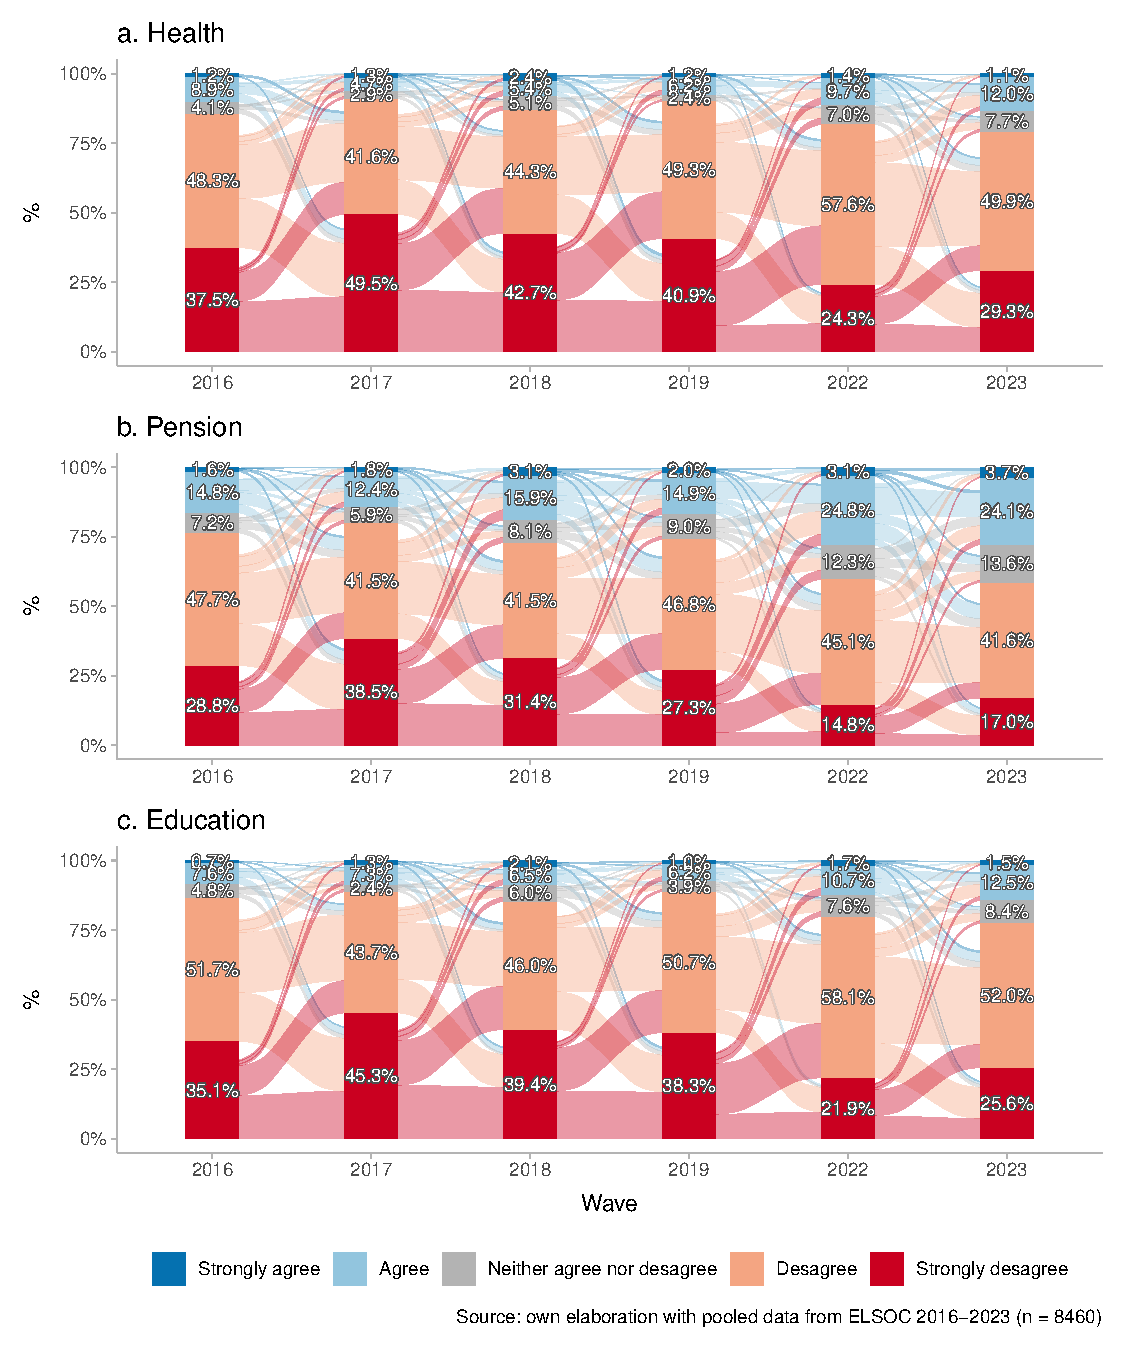
\includegraphics[width=1\textwidth,height=\textheight]{paper_files/figure-pdf/fig-alluvial-1.pdf}

}

\end{figure}%

Regarding the main dependent and independent variables of this study,
Figure~\ref{fig-meanchange} depicts their average changes over the
years. We observe an increase in the average level of market justice
preferences in the most recent waves, which begins in 2019. The highest
average consistently appears for perceived economic inequality, although
this variable shows a downward trend of roughly one point over time.
Interestingly, while perceptions of economic inequality declined in the
latest measurements (2022--2023), market justice preferences increased.
The meritocracy measures remain stable, though the perception that
individuals are rewarded for intelligence is slightly higher than the
perception that they are rewarded for their effort.

\begin{figure}[H]

\caption{\label{fig-meanchange}Change in the mean of market justice
preferences, economic inequality perception, and meritocracy
(2016-2023)}

\centering{

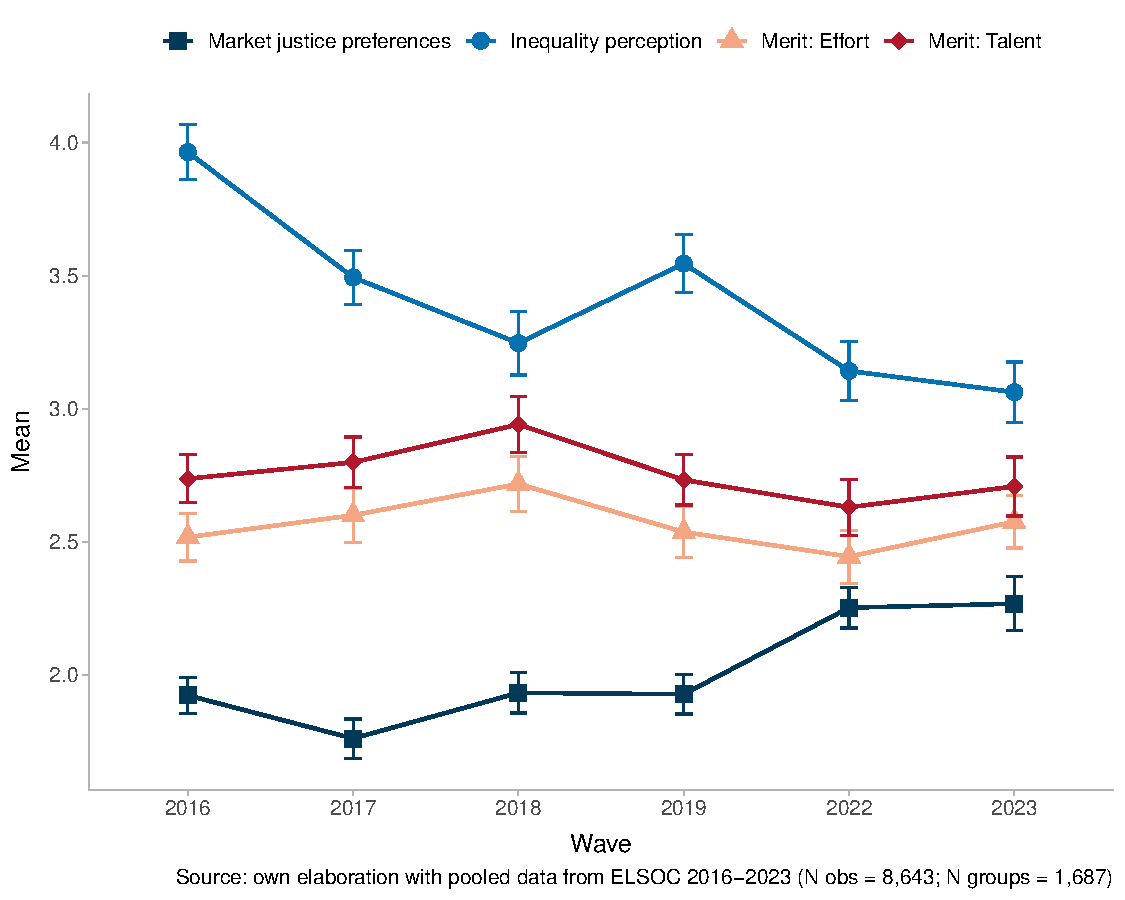
\includegraphics[width=1\textwidth,height=\textheight]{paper_files/figure-pdf/fig-meanchange-1.pdf}

}

\end{figure}%

Figure~\ref{fig-matrix} presents the correlation matrix for the main
variables in the latest wave (2023). Overall, the coefficients range
from low to moderate. The association between market justice preferences
and economic inequality perception is negative but small and
statistically significant (\(r\) = -0.05, \(p\) \textless{} .05). By
contrast, market justice preferences positively and significantly
correlate with the two meritocracy variables (\(r\) = 0.15, \(p\)
\textless{} .01; \(r\) = 0.13, \(p\) \textless{} .01). Perceived
economic inequality has negative and nonsignificant correlations with
both meritocracy perceptions (\(r\) = -0.04, \(p\) \textgreater{} .05;
\(r\) = -0.04, \(p\) \textgreater{} .05). Finally, the two meritocracy
variables exhibit a strong positive association with each other (\(r\) =
0.69, \(p\) \textless{} .01).

\begin{figure}[H]

\caption{\label{fig-matrix}Correlation matrix of the main variables for
the last wave (2023)}

\centering{

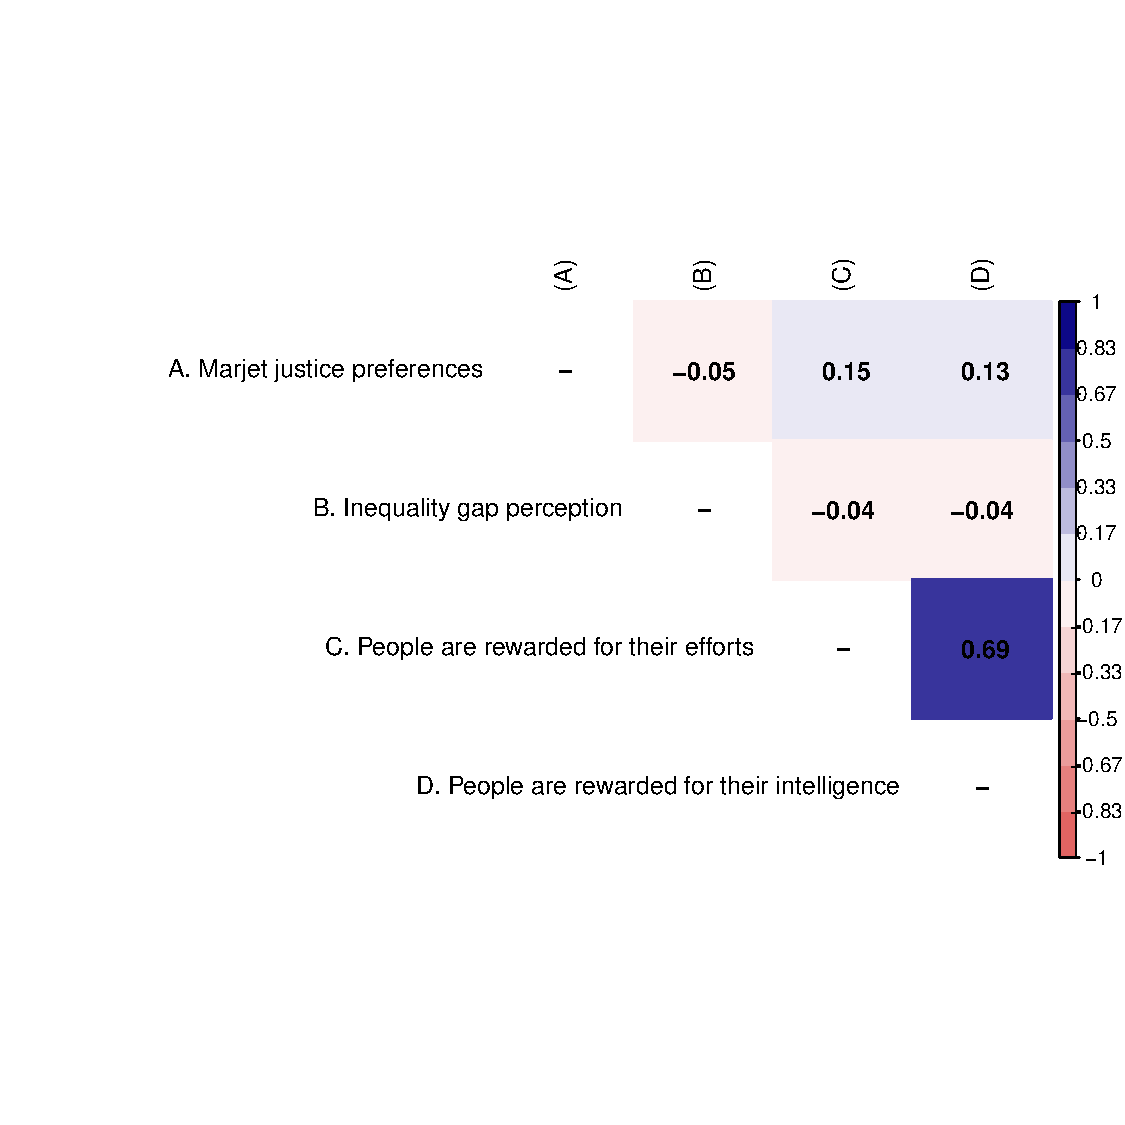
\includegraphics[width=0.9\textwidth,height=\textheight]{paper_files/figure-pdf/fig-matrix-1.pdf}

}

\end{figure}%

\subsection{Multilevel models}\label{multilevel-models}

Table~\ref{tbl-modelos} presents the results of the multilevel models
estimated for market justice preferences, examining both individuals
(within) and group-level (between) effects. The intraclass correlation
(\citeproc{ref-hoxMultilevelAnalysisTechniques2017a}{Hox et al., 2017})
from the empty model (see Supplementary Material), which decomposes the
variance of market justice preferences, is 0.23, indicating that
approximately 23\% of the variation is attributable to differences
between individuals. Complementary, 77\% of the variation corresponds to
within-individual differences over time.

\begin{table}

\caption{\label{tbl-modelos}Longitudinal multilevel models for market
justice preferences}

\centering{

~

Model 1

Model 2

Model 3

Model 4

Model 5

Model 6

Model 7

Intercept

1.968***

2.015***

2.030***

2.028***

2.169***

1.456***

1.547***

~

(0.021)

(0.035)

(0.035)

(0.035)

(0.070)

(0.097)

(0.115)

Wave (Ref.= 2016)

~

~

~

~

~

~

~

~

~

~

~

~

~

~

~

~~~~~Wave 2017

-0.167***

~

~

~

~

~

~

~

(0.027)

~

~

~

~

~

~

~~~~~Wave 2018

-0.025

~

~

~

~

~

~

~

(0.027)

~

~

~

~

~

~

~~~~~Wave 2019

-0.046

~

~

~

~

~

~

~

(0.027)

~

~

~

~

~

~

~~~~~Wave 2022

0.285***

~

~

~

~

~

~

~

(0.028)

~

~

~

~

~

~

~~~~~Wave 2023

0.284***

~

~

~

~

~

~

~

(0.027)

~

~

~

~

~

~

Wave

~

-0.121***

-0.125***

-0.128***

-0.128***

-0.128***

-0.129***

~

~

(0.022)

(0.022)

(0.022)

(0.022)

(0.022)

(0.022)

Wave\^{}2

~

0.028***

0.028***

0.029***

0.029***

0.029***

0.029***

~

~

(0.003)

(0.003)

(0.003)

(0.003)

(0.003)

(0.003)

Perception inequality (WE)

~

~

-0.039***

-0.034***

-0.034***

-0.034***

-0.034***

~

~

~

(0.010)

(0.010)

(0.010)

(0.010)

(0.010)

Merit: Effort (WE)

~

~

~

0.070***

0.070***

0.069***

0.069***

~

~

~

~

(0.012)

(0.012)

(0.012)

(0.012)

Merit: Talent (WE)

~

~

~

0.027*

0.027*

0.027*

0.027*

~

~

~

~

(0.012)

(0.012)

(0.012)

(0.012)

Perception inequality (BE)

~

~

~

~

-0.042*

-0.006

-0.033

~

~

~

~

~

(0.018)

(0.018)

(0.018)

Merit: Effort (BE)

~

~

~

~

~

0.186***

0.178***

~

~

~

~

~

~

(0.032)

(0.031)

Merit: Talent (BE)

~

~

~

~

~

0.040

0.019

~

~

~

~

~

~

(0.032)

(0.031)

Controls

No

No

No

No

No

No

Yes

BIC

20780.594

20780.617

20781.113

20726.753

20736.627

20655.172

20749.047

Numb. obs.

8643

8643

8643

8643

8643

8643

8643

Num. groups: individuals

1687

1687

1687

1687

1687

1687

1687

Var: individuals (Intercept)

0.172

0.223

0.219

0.209

0.207

0.182

0.171

Var: Residual

0.530

0.499

0.498

0.495

0.495

0.495

0.495

Var: individuals, wave

~

0.011

0.010

0.009

0.009

0.009

0.009

Cov: individuals (Intercept), wave

~

-0.025

-0.024

-0.021

-0.020

-0.019

-0.019

Note: Cells contain regression coefficients with standard errors in
parentheses. ***p \textless{} 0.001; **p \textless{} 0.01; *p
\textless{} 0.05.

}

\end{table}%

According to Model 1, which includes the survey waves to capture
intertemporal variations in the dependent variable, there is a decrease
in 2017 (\(\beta\) = -0.167, \(p\) \textless{} .001) relative to 2016,
and similarly in 2018 (\(\beta\) = -0.025, \(p\) \textgreater{} .05) and
2019 (\(\beta\) = -0.046, \(p\) \textgreater{} .05), although the latter
effects are not statistically significant. In contrast, in the more
recent waves of 2022 and 2023, there is a statistically significant
increase in market justice preferences (\(\beta\) = 0.285, \(p\)
\textless{} .001; \(\beta\) = 0.284, \(p\) \textless{} .001), suggesting
a non-linear effect. To model this trajectory over time, Model 2
incorporates time (survey waves) as a continuous variable, along with
its quadratic term, representing the non-linear association initially
observed in Model 1. While the linear term (survey wave) shows a
negative association, reflecting an overall decline in market
preferences over time, the positive quadratic term indicates a reversal
of this pattern in the final measurement points.

Models 3 and 4 incorporate the within-group effects (WE) of the primary
independent variables, capturing how individual changes in these
variables over time shape the dependent variable. The results in Model 3
suggest that the within effect of perceived economic inequality is
negative and statistically significant (\(p\) \textless{} .001).
Specifically, each one-point increase in an individual's perception of
economic inequality between waves is associated with a 0.034 point
decrease in market justice preferences. Model 4 shows that meritocratic
beliefs operate in the opposite direction. An upward shift in the
perception that effort is rewarded exerts a positive within effect
(\(\beta\) = 0.071, \(p\) \textless{} .001), and a parallel increase in
the perception that intelligence and ability are rewarded is likewise
associated with higher market-justice preferences (\(\beta\) = 0.028,
\(p\) \textless{} .05). Taken together, these results suggest that
individuals who increasingly perceive meritocracy---whether through
effort or talent---tend to hold stronger market justice preferences.

When examining the between-group effects (BE) in Model 5 and 6, which
capture differences between individuals in the average of the main
variables, a similar pattern emerges. Individuals who perceive higher
levels of economic inequality tend to prefer less market justice
(\(\beta\) = -0.042, \(p\) \textless{} .05). In Model 6, the
meritocratic perception that effort is rewarded is positively associated
with market justice preferences (\(\beta\) = 0.186, \(p\) \textless{}
.001), whereas the perception that talent is rewarded shows a positive
but non-significant coefficient (\(\beta\) = 0.040). Notably, once the
meritocratic variables are included, the negative coefficient for
perceived economic inequality remains but is no longer statistically
significant.

Model 7 adds the control variables. With the exception of the
between-effect for perceived economic inequality---which becomes
nonsignificant---the within- and between-effects of the principal
predictors retain both their direction and statistical significance,
confirming the robustness of the associations (see Supplementary
Material for effects of control variables).

\begin{table}

\caption{\label{tbl-interactions1}Interactions for meritocracy,
perceived economic inequality and market justice preferences}

\centering{

~

Model 8

Model 9

Model 10

Model 11

Intercept

1.561***

1.555***

2.187***

2.340***

~

(0.115)

(0.115)

(0.265)

(0.281)

Perception inequality (WE)

-0.035***

-0.035***

-0.035***

-0.035***

~

(0.010)

(0.010)

(0.010)

(0.010)

Merit: Effort (WE)

0.072***

0.074***

0.073***

0.073***

~

(0.013)

(0.012)

(0.012)

(0.012)

Merit: Talent (WE)

0.031*

0.031*

0.030*

0.030*

~

(0.012)

(0.013)

(0.012)

(0.012)

Perception inequality (BE)

-0.032

-0.033

-0.213**

-0.255***

~

(0.018)

(0.018)

(0.073)

(0.077)

Merit: Effort (BE)

0.177***

0.173***

-0.062

0.179***

~

(0.032)

(0.031)

(0.097)

(0.032)

Merit: Talent (BE)

0.015

0.021

0.014

-0.266**

~

(0.031)

(0.031)

(0.031)

(0.099)

Merit: Effort (WE) x Perception inequality (WE)

0.017

~

~

~

~

(0.012)

~

~

~

Merit: Talent (WE) x Perception inequality (WE)

~

0.011

~

~

~

~

(0.012)

~

~

Merit: Effort (BE) x Perception inequality (BE)

~

~

0.072**

~

~

~

~

(0.028)

~

Merit: Talent (BE) x Perception inequality (BE)

~

~

~

0.082**

~

~

~

~

(0.027)

Controls

Yes

Yes

Yes

Yes

BIC

20842.694

20835.920

20808.677

20806.384

Numb. obs.

8643

8643

8643

8643

Num. groups: individuals

1687

1687

1687

1687

Var: individuals (Intercept)

0.145

0.145

0.141

0.141

Var: individuals, merit effort cwc

0.020

~

~

~

Var: individuals, perception inequality cwc

0.000

0.000

~

~

Cov: individuals (Intercept), merit effort cwc

0.004

~

~

~

Cov: individuals (Intercept), perception inequality cwc

-0.006

-0.005

~

~

Cov: individuals, merit effort cwc, perception inequality cwc

0.000

~

~

~

Var: Residuals

0.512

0.511

0.528

0.528

Var: individuals, merit talent cwc

~

0.020

~

~

Cov: individuals (Intercept), merit talent cwc

~

0.012

~

~

Cov: individuals, merit talent cwc, perception inequality cwc

~

0.001

~

~

Note: Cells contain regression coefficients with standard errors in
parentheses. ***p \textless{} 0.001; **p \textless{} 0.01; *p
\textless{} 0.05. CWC = centered within group.

}

\end{table}%

\begin{figure}[H]

\caption{\label{fig-interact}Between effects of meritocratic perceptions
on market justice preferences by economic inequality perception}

\centering{

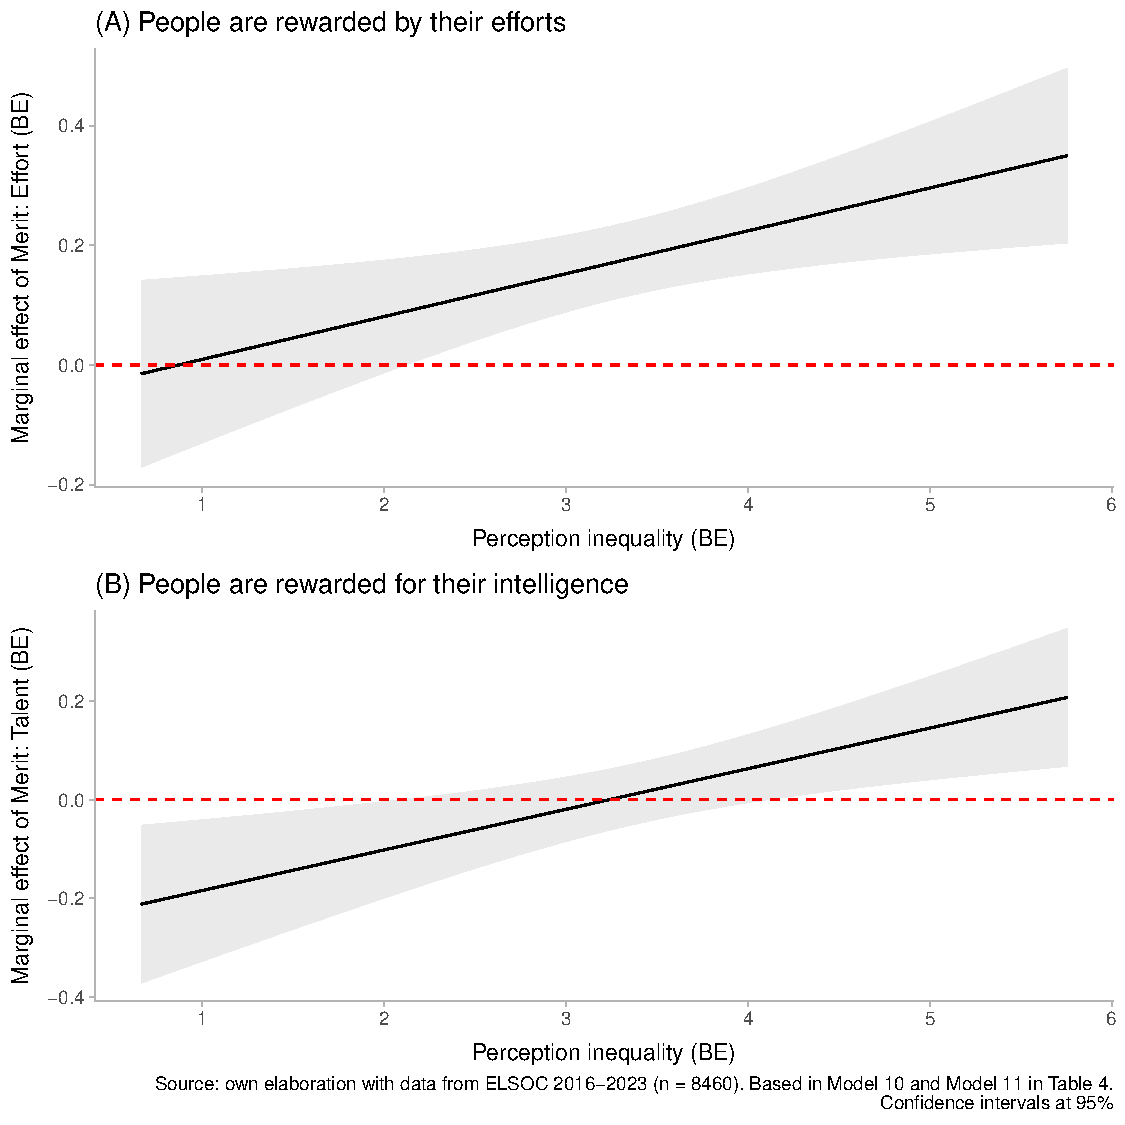
\includegraphics[width=1\textwidth,height=\textheight]{paper_files/figure-pdf/fig-interact-1.pdf}

}

\end{figure}%

Table~\ref{tbl-interactions1} examines whether perceived economic
inequality moderates the effect of meritocratic beliefs on market
justice preferences. Contrary to our hypothesis, the interaction terms
in the within-person specification (Models 8 and 9) do not reach
statistical significance. However, in the between-person specification
(Models 10 and 11), the interaction terms are statistically significant,
suggesting that perceptions of economic inequality meaningfully alter
the effect of meritocracy on support for market-based allocation of
social services. These positive effects indicate that, as perceptions of
inequality increase, the positive association between meritocratic
perceptions and market justice preferences becomes stronger. The
marginal effects of this interaction are illustrated in
Figure~\ref{fig-interact}, which shows that the effect of meritocratic
perceptions on market justice preferences intensifies as perceived
economic inequality rises.

\begin{table}

\caption{\label{tbl-interactions2}Interactions for meritocracy,
perceived economic inequality and market justice preferences}

\centering{

~

Model 12

Model 13

Model 14

Model 15

Model 16

Model 17

Intercept

1.543***

1.527***

1.521***

1.680***

1.374***

1.362***

~

(0.115)

(0.114)

(0.114)

(0.139)

(0.133)

(0.134)

Wave x Perception inequality (WE)

-0.004

~

~

~

~

~

~

(0.006)

~

~

~

~

~

Wave x Merit: effort (WE)

~

-0.008

~

~

~

~

~

~

(0.006)

~

~

~

~

Wave x Merit: talent (WE)

~

~

-0.006

~

~

~

~

~

~

(0.006)

~

~

~

Wave x Perception inequality (BE)

~

~

~

0.011

~

~

~

~

~

~

(0.007)

~

~

Wave x Merit: effort (BE)

~

~

~

~

-0.021*

~

~

~

~

~

~

(0.008)

~

Wave x Merit: talent (BE)

~

~

~

~

~

-0.020*

~

~

~

~

~

~

(0.008)

Controls

Yes

Yes

Yes

Yes

Yes

Yes

BIC

20792.207

20767.371

20754.324

20782.059

20749.596

20754.417

Numb. obs.

8643

8643

8643

8643

8643

8643

Num. groups: individuals

1687

1687

1687

1687

1687

1687

Var: individuals (Intercept)

0.176

0.167

0.168

0.383

0.254

0.010

Var: individuals, perception inequality cwc

0.000

~

~

~

~

~

Var: individuals, wave

0.010

0.009

0.009

0.009

0.009

0.009

Cov: individuals (Intercept), perception inequality cwc

-0.007

~

~

~

~

~

Cov: individuals (Intercept), wave

-0.021

-0.018

-0.018

-0.048

-0.003

0.006

Cov: individuals, perception inequality cwc, wave

0.002

~

~

~

~

~

Var: Residuals

0.495

0.480

0.479

0.494

0.494

0.494

Var: individuals, merit effort cwc

~

0.019

~

~

~

~

Cov: individuals (Intercept), merit effort cwc

~

0.023

~

~

~

~

Cov: individuals, merit effort cwc, wave

~

-0.005

~

~

~

~

Var: individuals, merit talent cwc

~

~

0.019

~

~

~

Cov: individuals (Intercept), merit talent cwc

~

~

0.034

~

~

~

Cov: individuals, merit talent cwc, wave

~

~

-0.006

~

~

~

Var: individuals, perception inequality mean

~

~

~

0.008

~

~

Cov: individuals (Intercept), perception inequality mean

~

~

~

-0.045

~

~

Cov: individuals, perception inequality mean, wave

~

~

~

0.009

~

~

Var: individuals, merit effort mean

~

~

~

~

0.053

~

Cov: individuals (Intercept), merit effort mean

~

~

~

~

-0.089

~

Cov: individuals, merit effort mean, wave

~

~

~

~

-0.006

~

Var: individuals, merit talent mean

~

~

~

~

~

0.025

Cov: individuals (Intercept), merit talent mean

~

~

~

~

~

-0.007

Cov: individuals, merit talent mean, wave

~

~

~

~

~

-0.009

Note: Cells contain regression coefficients with standard errors in
parentheses. ***p \textless{} 0.001; **p \textless{} 0.01; *p
\textless{} 0.05. CWC = centered within group.

}

\end{table}%

With respect to the temporal dynamics of the key predictors,
Table~\ref{tbl-interactions2} shows that time only has significant
effects on the between effects of the meritocratic variables. These
interaction effects are negative and mean that in the last waves, the
impact of meritocratic variables on market justice preferences is
attenuated. Specifically, as time advances, the positive within-person
effect of perceiving that effort is rewarded (Model 16) or that
intelligence is rewarded (Model 17) progressively attenuates. Put
differently, the uplift in market justice preferences associated with a
strong meritocratic perception becomes smaller in each successive wave.

\section{Discussion}\label{discussion}

This study tests several key hypotheses concerning the relationships
between perceptions of economic inequality, meritocratic beliefs, and
attitudes toward market justice in Chile. It posits that higher
perceived inequality and stronger meritocratic beliefs both
independently contribute to greater support for market-based
distributions of social goods. Furthermore, the study examines how
perceived economic inequality moderates the influence of meritocratic
beliefs on market justice preferences. Additionally, it considers how
major social and political mobilizations, such as those occurring around
2019 and subsequent years, may have weakened these relationships,
reflecting increased critical perspectives on systemic inequalities and
market mechanisms. The subsequent discussion interprets the empirical
findings in light of these hypotheses, considering their implications
for understanding attitudes toward inequality and social justice in a
context marked by profound social change.

The first hypothesis suggested that perceptions of economic inequality
were strongly linked to attitudes toward market justice. The findings
demonstrated that individuals perceiving higher income disparities
showed stronger support for the distribution of social services based on
individual income, aligning with theories emphasizing that awareness of
inequality could fuel a critical view of such policies
(\citeproc{ref-Castillo2012a_justice}{Castillo, 2012};
\citeproc{ref-mijs_paradox_2021}{Mijs, 2021}). This relationship
reflected a moral economy where perceptions of systemic unfairness
threatened the legitimacy of existing distributions, prompting calls for
greater equity. Interestingly, the negative within-effects observed over
time implied that as perceptions of inequality became more salient, some
individuals experienced a decline in support for market justice,
possibly due to increasing distrust in market mechanisms or
disillusionment with the fairness of the system. This indicated that
while perception heightened awareness, prolonged exposure or social
mobilization could also foster skepticism about whether redistribution
effectively addressed inequality or simply perpetuated systemic flaws.

Regarding the second hypothesis, the results reinforced that
meritocratic perceptions ---particularly those emphasizing individual
effort and talent--- were associated with stronger support for
market-based distribution systems. Individuals who viewed success as
primarily earned through effort were more inclined to justify existing
inequalities, seeing them as outcomes of individual merit rather than
systemic injustice. This aligned with research indicating that
meritocratic narratives served as moral justifications that reinforced
societal stratification (\citeproc{ref-Castillo2012a_justice}{Castillo,
2012}; \citeproc{ref-hoyt_mindsets_2023}{Hoyt et al., 2023}). These
beliefs functioned symbolically to legitimize structural disparities,
reducing support for redistributive measures by framing inequality as
fair and deserved. The findings suggested that these perceptions
bolstered the social hierarchy by fostering acceptance of inequality as
a reflection of individual virtue rather than structural failure, which
was especially pertinent in neoliberal contexts like Chile's, where
market logic heavily influenced social attitudes
(\citeproc{ref-canalesceron_sujeto_2021}{Canales Cerón et al., 2021}).

The third hypothesis concerned the moderating role of perceptions of
inequality on the relationship between meritocracy and market justice
attitudes. The analysis indicated that the positive association between
meritocratic beliefs and support for market-based distribution tended to
weaken when perceptions of economic inequality were particularly high.
Although this moderation is not significant for within-subject effects
(i.e.~over time), when taking into account between-subjects differences
we found a positive effect. This appears as contrary to our initial
hypothesis, as it would mean that effect of meritocratic perceptions
becomes stronger as perception of inequality increases. Nevertheless, we
need to be cautious about this interpretation, as the main effect of
inequality perception on market justice is negative. Therefore, as
perceived inequality become less negative (i.e.~more positive), or
closer to zero, then the meritocratic perception has an stronger
positive relationship on market justice preferences. This could mean
that meritocratic perceptions play an stronger role in justification of
market justice inequalities for those who are less capable or less prone
to perceive inequality.

Finally, the fourth hypothesis addressed the impact of recent social
movements, particularly from 2019 onwards, on the relationship between
meritocratic beliefs, perceptions of inequality, and attitudes toward
market justice. The results suggested that these movements contributed
to a more critical stance toward the fairness of existing distributional
mechanisms. Post-mobilization, the positive relationship between
meritocratic beliefs and support for inequality appeared attenuated,
indicating that collective action and public discourse during this
period fostered questioning of the legitimacy of systemic inequalities
justified solely through meritocratic narratives. These social
mobilizations challenged dominant narratives, emphasizing structural
barriers and systemic injustices, which in turn weakened the association
between individual effort and deservingness. This is aligned with
literature emphasizing that social protests act as catalysts for
transforming societal attitudes by disrupting normative beliefs and
encouraging more critical evaluations of institutional legitimacy
(\citeproc{ref-tilly_contentious_2015}{Tilly \& Tarrow, 2015}). The
findings underscored the importance of socio-political context in
shaping and reshaping attitudes toward inequality and justice,
highlighting how collective action could temporarily or permanently
alter the normative foundations that sustained support for market
justice.

\section{Conclusions}\label{conclusions}

This study examined the complex interplay between perceptions of
economic inequality, meritocratic beliefs, and attitudes toward market
justice in Chile from 2016 to 2023, drawing on longitudinal data from
the ELSOC survey. By exploring how subjective assessments and social
contexts influence support for redistribution and market-based resource
allocation, the research offers different elements that contribute to
the understanding of the normative foundations underpinning social
justice attitudes in a highly unequal, neoliberal environment.

The findings confirm that higher perceptions of economic inequality are
associated with less support for market justice attitudes, this is, the
belief that it is fine that those with higher income have better social
services such as education, pensions and health. Meritocratic beliefs
strongly reinforce support for market justice, serving as moral
justifications for structural inequalities. Additionally, perceptions of
inequality moderate the influence of meritocratic beliefs, such that as
the awareness of disparities are attenuated (i.e.~less negative) the
role of meritocratic beliefs on existing market-based allocations become
stronger. Notably, the social mobilizations of 2019 and subsequent
periods seem to have contributed to shifting attitudes, fostering
greater skepticism of systemic fairness and reducing the legitimizing
power of meritocratic narratives.

This research advances the extant literature by integrating subjective
perceptions with social and political contexts to explain attitudes
toward economic inequality and distributional justice. While previous
studies primarily focused on objective measures or individual
characteristics, this work emphasizes the dynamic and interactional
nature of perceptions and beliefs over time. It highlights the
importance of socio-political upheavals in reshaping normative
attitudes, underscoring the role of collective action in challenging
entrenched narratives of meritocracy and fairness. The longitudinal
approach provides a deeper temporal perspective on how societal events
could influence individual beliefs and preferences.

Despite its contributions, the study has several limitations. First, the
reliance on self-reported perceptions and attitudes may be subject to
social desirability bias. Second, the focus on Chile, while offering
valuable insights into a specific context, limits the generalizability
of results to other countries with different institutional and cultural
backgrounds. Third, the observational nature of the data prevents causal
inferences, and unobserved confounding factors may influence the
observed relationships. Finally, the potential influence of media,
political discourse, and peer effects on perceptions was not directly
assessed. Future research could explore the causal mechanisms linking
perceptions and attitudes, possibly through experimental or mixed-method
designs. Comparative studies across different national contexts would
help determine the universality or specificity of these dynamics.
Additionally, investigating the role of media, political communication,
and education in shaping perceptions of inequality and meritocracy would
deepen understanding of the normative foundations of social justice
attitudes. Finally, examining how these perceptions influence behavioral
outcomes, such as political participation or support for social
movements, would provide valuable insights into the pathways from
beliefs to collective action and policy change.

\section{References}\label{references}

\phantomsection\label{refs}
\begin{CSLReferences}{1}{0}
\bibitem[\citeproctext]{ref-akyelken_urban_2020}
Akyelken, N. (2020). Urban conceptions of economic inequalities.
\emph{Regional Studies}, \emph{54}(6), 863--872.
\url{https://doi.org/10.1080/00343404.2020.1732902}

\bibitem[\citeproctext]{ref-auspurg_why_2017}
Auspurg, K., Hinz, T., \& Sauer, C. (2017). Why {Should Women Get Less}?
{Evidence} on the {Gender Pay Gap} from {Multifactorial Survey
Experiments}. \emph{American Sociological Review}, \emph{82}(1),
179--210. \url{https://doi.org/10.1177/0003122416683393}

\bibitem[\citeproctext]{ref-bates_fitting_2015}
Bates, D., Mächler, M., Bolker, B., \& Walker, S. (2015). Fitting linear
mixed-effects models using {lme4}. \emph{Journal of Statistical
Software}, \emph{67}(1), 1--48.
\url{https://doi.org/10.18637/jss.v067.i01}

\bibitem[\citeproctext]{ref-batruch_belief_2023}
Batruch, A., Jetten, J., Van De Werfhorst, H., Darnon, C., \& Butera, F.
(2023). Belief in {School Meritocracy} and the {Legitimization} of
{Social} and {Income Inequality}. \emph{Social Psychological and
Personality Science}, \emph{14}(5), 621--635.
\url{https://doi.org/10.1177/19485506221111017}

\bibitem[\citeproctext]{ref-boccardo_30_2020}
Boccardo, G. (2020). \emph{30 a{ñ}os de privatizaciones en {Chile}: Lo
que la pandemia revel{ó}} (Nodo XXI). Santiago.

\bibitem[\citeproctext]{ref-busemeyer_positive_2021}
Busemeyer, M. R., Abrassart, A., \& Nezi, R. (2021). Beyond {Positive}
and {Negative}: {New Perspectives} on {Feedback Effects} in {Public
Opinion} on the {Welfare State}. \emph{British Journal of Political
Science}, \emph{51}(1), 137--162.
\url{https://doi.org/10.1017/S0007123418000534}

\bibitem[\citeproctext]{ref-canalesceron_sujeto_2021}
Canales Cerón, M., Orellana Calderón, V. S., \& Guajardo Mañán, F.
(2021). Sujeto y cotidiano en la era neoliberal: El caso de la
educaci{ó}n chilena. \emph{Revista Mexicana de Ciencias Pol{í}ticas y
Sociales}, \emph{67}(244).
\url{https://doi.org/10.22201/fcpys.2448492xe.2022.244.70386}

\bibitem[\citeproctext]{ref-castillo_cual_2009}
Castillo, J. C. (2009). {{\textquestiondown}Cu{á}l es la brecha salarial
justa? Opini{ó}n p{ú}blica y legitimaci{ó}n de la desigualdad en Chile}.
\emph{Estudios P{ú}blicos}, (113).

\bibitem[\citeproctext]{ref-Castillo2011}
Castillo, J. C. (2011). Legitimacy of {Inequality} in a {Highly Unequal
Context}: {Evidence} from the {Chilean Case}. \emph{Social Justice
Research}, \emph{24}(4), 314--340.
\url{https://doi.org/10.1007/s11211-011-0144-5}

\bibitem[\citeproctext]{ref-Castillo2012a_justice}
Castillo, J. C. (2012). Is {Inequality Becoming Just}? {Changes} in
{Public Opinion} about {Economic Distribution} in {Chile}.
\emph{Bulletin of Latin American Research}, \emph{31}(1), 1--18.
\url{https://doi.org/10.1111/j.1470-9856.2011.00605.x}

\bibitem[\citeproctext]{ref-castillo_perception_2022}
Castillo, J. C., García-Castro, J.-D., \& Venegas, M. (2022). Perception
of economic inequality: Concepts, associated factors and prospects of a
burgeoning research agenda. \emph{International Journal of Social
Psychology}, \emph{37}(1), 180--207.
\url{https://doi.org/10.1080/02134748.2021.2009275}

\bibitem[\citeproctext]{ref-castillo_multidimensional_2023}
Castillo, J. C., Iturra, J., Maldonado, L., Atria, J., \& Meneses, F.
(2023). A {Multidimensional Approach} for {Measuring Meritocratic
Beliefs}: {Advantages}, {Limitations} and {Alternatives} to the {ISSP
Social Inequality Survey}. \emph{International Journal of Sociology},
1--25. \url{https://doi.org/10.1080/00207659.2023.2274712}

\bibitem[\citeproctext]{ref-castillo_percepcion_2019}
Castillo, J. C., Miranda, D., \& Carrasco, D. (2012). Percepci{ó}n de
{Desigualdad Econ{ó}mica} en {Chile}: {Medici{ó}n}, {Diferencias} y
{Determinantes}. \emph{Psykhe (Santiago)}, \emph{21}(1), 99--114.
\url{https://doi.org/10.4067/S0718-22282012000100007}

\bibitem[\citeproctext]{ref-castillo_socialization_2024}
Castillo, J. C., Salgado, M., Carrasco, K., \& Laffert, A. (2024). The
{Socialization} of {Meritocracy} and {Market Justice Preferences} at
{School}. \emph{Societies}, \emph{14}(11), 214.
\url{https://doi.org/10.3390/soc14110214}

\bibitem[\citeproctext]{ref-chancel_world_2022}
Chancel, L., Piketty, T., Saez, E., \& Zucman, G. (2022). World
inequality report 2022.
https://bibliotecadigital.ccb.org.co/handle/11520/27510.

\bibitem[\citeproctext]{ref-davis_principles_2001}
Davis, K., \& Moore, W. E. (2001). Some {Principles} of
{Stratification}. In \emph{Social {Stratification}, {Class}, {Race}, and
{Gender} in {Sociological Perspective}, {Second Edition}} (2nd ed.).
Routledge.

\bibitem[\citeproctext]{ref-easterbrook_social_2021}
Easterbrook, M. J. (2021). \emph{The social psychology of economic
inequality} (43rd ed., Vol. 2021). UNU-WIDER.
\url{https://doi.org/10.35188/UNU-WIDER/2021/981-5}

\bibitem[\citeproctext]{ref-elsoc_estudio_2022}
ELSOC, S. T. (2022). Estudio {Longitudinal Social} de {Chile}. Harvard
Dataverse. \url{https://doi.org/10.7910/dvn/0kirbj}

\bibitem[\citeproctext]{ref-engelhardt_what_2018}
Engelhardt, C., \& Wagener, A. (2018). What do {Germans} think and know
about income inequality? {A} survey experiment. \emph{Socio-Economic
Review}, \emph{16}(4), 743--767.
\url{https://doi.org/10.1093/ser/mwx036}

\bibitem[\citeproctext]{ref-flores_top_2020}
Flores, I., Sanhueza, C., Atria, J., \& Mayer, R. (2020). Top {Incomes}
in {Chile}: {A Historical Perspective} on {Income Inequality},
1964--2017. \emph{Review of Income and Wealth}, \emph{66}(4), 850--874.
\url{https://doi.org/10.1111/roiw.12441}

\bibitem[\citeproctext]{ref-garcia-castro_perceiving_2020}
García-Castro, J. D., Rodríguez-Bailón, R., \& Willis, G. B. (2020).
Perceiving economic inequality in everyday life decreases tolerance to
inequality. \emph{Journal of Experimental Social Psychology}, \emph{90},
104019. \url{https://doi.org/10.1016/j.jesp.2020.104019}

\bibitem[\citeproctext]{ref-garcia-sanchez_creencias_2022}
García-Sánchez, E., \& De Carvalho, S. (2022). Las creencias que
justifican la desigualdad moderan la relaci{ó}n entre el estatus
socioecon{ó}mico y el apoyo a la redistribuci{ó}n. \emph{Revista
Internacional de Sociolog{í}a}, \emph{80}(3), e210.
\url{https://doi.org/10.3989/ris.2022.80.3.21.29}

\bibitem[\citeproctext]{ref-garcia-sanchez_attitudes_2020}
García-Sánchez, E., Osborne, D., Willis, G. B., \& Rodríguez-Bailón, R.
(2020). Attitudes towards redistribution and the interplay between
perceptions and beliefs about inequality. \emph{British Journal of
Social Psychology}, \emph{59}(1), 111--136.
\url{https://doi.org/10.1111/bjso.12326}

\bibitem[\citeproctext]{ref-garcia-sanchez_vicious_2019}
García-Sánchez, E., Van Der Toorn, J., Rodríguez-Bailón, R., \& Willis,
G. B. (2019). The {Vicious Cycle} of {Economic Inequality}: {The Role}
of {Ideology} in {Shaping} the {Relationship Between} {``{What Is}''}
and {``{What Ought} to {Be}''} in 41 {Countries}. \emph{Social
Psychological and Personality Science}, \emph{10}(8), 991--1001.
\url{https://doi.org/10.1177/1948550618811500}

\bibitem[\citeproctext]{ref-garcia-sanchez_perceptions_2018}
García-Sánchez, E., Willis, G. B., Rodríguez-Bailón, R., Palacio Sañudo,
J., David Polo, J., \& Rentería Pérez, E. (2018). Perceptions of
{Economic Inequality} and {Support} for {Redistribution}: {The} role of
{Existential} and {Utopian Standards}. \emph{Social Justice Research},
\emph{31}(4), 335--354. \url{https://doi.org/10.1007/s11211-018-0317-6}

\bibitem[\citeproctext]{ref-gijsberts_thelegitimation_1999}
Gijsberts, M. (1999). \emph{{Thelegitimation of inequality in state-
socialist and market societies, 1987 - 1996}}. Amsterdam: Thela Thesis.

\bibitem[\citeproctext]{ref-gimpelson_misperceiving_2018}
Gimpelson, V., \& Treisman, D. (2018). Misperceiving inequality.
\emph{Economics \& Politics}, \emph{30}(1), 27--54.
\url{https://doi.org/10.1111/ecpo.12103}

\bibitem[\citeproctext]{ref-hadler_why_2005}
Hadler, M. (2005). Why {Do People Accept Different Income Ratios}?: {A
Multi-level Comparison} of {Thirty Countries}. \emph{Acta Sociologica},
\emph{48}(2), 131--154. \url{https://doi.org/10.1177/0001699305053768}

\bibitem[\citeproctext]{ref-hoxMultilevelAnalysisTechniques2017a}
Hox, J. J., Moerbeek, M., \& Van de Schoot, R. (2017). \emph{Multilevel
{Analysis}: {Techniques} and {Applications}}.

\bibitem[\citeproctext]{ref-hoyt_mindsets_2023}
Hoyt, C. L., Burnette, J. L., Billingsley, J., Becker, W., \& Babij, A.
D. (2023). Mindsets of poverty: {Implications} for redistributive policy
support. \emph{Analyses of Social Issues and Public Policy},
\emph{23}(3), 668--693. \url{https://doi.org/10.1111/asap.12367}

\bibitem[\citeproctext]{ref-immergut_it_2020}
Immergut, E. M., \& Schneider, S. M. (2020). Is it unfair for the
affluent to be able to purchase {``better''} healthcare? {Existential}
standards and institutional norms in healthcare attitudes across 28
countries. \emph{Social Science \& Medicine}, \emph{267}, 113146.
\url{https://doi.org/10.1016/j.socscimed.2020.113146}

\bibitem[\citeproctext]{ref-janmaat_subjective_2013}
Janmaat, J. G. (2013). Subjective inequality: {A} review of
international comparative studies on people's views about inequality.
\emph{Archives Europeennes de Sociologie}, \emph{54}(3), 357--389.
\url{https://doi.org/10.1017/S0003975613000209}

\bibitem[\citeproctext]{ref-kluegel_social_1995a}
Kluegel, J. R., Mason, D. S., \& Wegener, B. (Eds.). (1995).
\emph{Social {Justice} and {Political Change}: {Public Opinion} in
{Capitalist} and {Post-Communist States}} (1st ed.). Routledge.

\bibitem[\citeproctext]{ref-kluegel_legitimation_1999}
Kluegel, J. R., Mason, D. S., \& Wegener, B. (1999). The {Legitimation}
of {Capitalism} in the {Postcommunist Transition}: {Public Opinion}
about {Market Justice}, 1991-1996. \emph{European Sociological Review},
\emph{15}(3), 251--283. Retrieved from
\url{https://www.jstor.org/stable/522731}

\bibitem[\citeproctext]{ref-kluegel_beliefs_1981}
Kluegel, J. R., \& Smith, E. R. (1981). Beliefs {About Stratification}.
\emph{Annual Review of Sociology}, 29--56.

\bibitem[\citeproctext]{ref-knell_perceptions_2020}
Knell, M., \& Stix, H. (2020). Perceptions of inequality. \emph{European
Journal of Political Economy}, \emph{65}, 101927.
\url{https://doi.org/10.1016/j.ejpoleco.2020.101927}

\bibitem[\citeproctext]{ref-koos_moral_2019}
Koos, S., \& Sachweh, P. (2019). The moral economies of market
societies: Popular attitudes towards market competition, redistribution
and reciprocity in comparative perspective. \emph{Socio-Economic
Review}, \emph{17}(4), 793--821.
\url{https://doi.org/10.1093/ser/mwx045}

\bibitem[\citeproctext]{ref-kuhn_eye_2011}
Kuhn, A. (2011). In the eye of the beholder: {Subjective} inequality
measures and individuals' assessment of market justice. \emph{European
Journal of Political Economy}, \emph{27}(4), 625--641.
\url{https://doi.org/10.1016/j.ejpoleco.2011.06.002}

\bibitem[\citeproctext]{ref-lane_market_1986}
Lane, R. E. (1986). Market {Justice}, {Political Justice}.
\emph{American Political Science Review}, \emph{80}(2), 383--402.
\url{https://doi.org/10.2307/1958264}

\bibitem[\citeproctext]{ref-lee_fairness_2023}
Lee, J.-S., \& Stacey, M. (2023). Fairness perceptions of educational
inequality: The effects of self-interest and neoliberal orientations.
\emph{The Australian Educational Researcher}.
\url{https://doi.org/10.1007/s13384-023-00636-6}

\bibitem[\citeproctext]{ref-lindh_public_2015}
Lindh, A. (2015). Public {Opinion} against {Markets}? {Attitudes}
towards {Market Distribution} of {Social Services} -- {A Comparison} of
17 {Countries}. \emph{Social Policy \& Administration}, \emph{49}(7),
887--910. \url{https://doi.org/10.1111/spol.12105}

\bibitem[\citeproctext]{ref-mijs_stratified_2016}
Mijs, J. (2016). Stratified {Failure}: {Educational Stratification} and
{Students}' {Attributions} of {Their Mathematics Performance} in 24
{Countries}. \emph{Sociology of Education}, \emph{89}(2), 137--153.
\url{https://doi.org/10.1177/0038040716636434}

\bibitem[\citeproctext]{ref-mijs_paradox_2021}
Mijs, J. (2021). The paradox of inequality: Income inequality and belief
in meritocracy go hand in hand. \emph{Socio-Economic Review},
\emph{19}(1), 7--35. \url{https://doi.org/10.1093/ser/mwy051}

\bibitem[\citeproctext]{ref-pedersen_attitudes_2019}
Pedersen, R. T., \& Mutz, D. C. (2019). Attitudes {Toward Economic
Inequality}: {The Illusory Agreement}. \emph{Political Science Research
and Methods}, \emph{7}(04), 835--851.
\url{https://doi.org/10.1017/psrm.2018.18}

\bibitem[\citeproctext]{ref-reynolds_perceptions_2014}
Reynolds, J., \& Xian, H. (2014). Perceptions of meritocracy in the land
of opportunity. \emph{Research in Social Stratification and Mobility},
\emph{36}, 121--137. \url{https://doi.org/10.1016/j.rssm.2014.03.001}

\bibitem[\citeproctext]{ref-sandel_tyranny_2020}
Sandel, M. J. (2020). \emph{The tyranny of merit: {What}'s become of the
common good?} (First edition). New York: {Farrar, Straus and Giroux}.

\bibitem[\citeproctext]{ref-schneider_poverty_2015}
Schneider, S. M., \& Castillo, J. C. (2015). Poverty {Attributions} and
the {Perceived Justice} of {Income Inequality} : {A Comparison} of
{East} and {West Germany}.
\url{https://doi.org/10.1177/0190272515589298}

\bibitem[\citeproctext]{ref-schroder_income_2017}
Schröder, M. (2017). Is {Income Inequality Related} to {Tolerance} for
{Inequality}? \emph{Social Justice Research}, \emph{30}(1), 23--47.
\url{https://doi.org/10.1007/s11211-016-0276-8}

\bibitem[\citeproctext]{ref-singer_applied_2009}
Singer, J. D., \& Willett, J. B. (2009). \emph{Applied longitudinal data
analysis: Modeling change and event occurence}. New York: Oxford
University Press, Incorporated.

\bibitem[\citeproctext]{ref-svallfors_political_2007}
Svallfors, S. (Ed.). (2007). \emph{The {Political Sociology} of the
{Welfare State}: {Institutions}, {Social Cleavages}, and {Orientations}}
(1st ed.). Stanford University Press.
\url{https://doi.org/10.2307/j.ctvr0qv0q}

\bibitem[\citeproctext]{ref-tejero-peregrina_perceived_2025}
Tejero-Peregrina, L., Willis, G., Sánchez-Rodríguez, Á., \&
Rodríguez-Bailón, R. (2025). From {Perceived Economic Inequality} to
{Support} for {Redistribution}: {The Role} of {Meritocracy Perception}.
\emph{International Review of Social Psychology}, \emph{38}(1), 4.
\url{https://doi.org/10.5334/irsp.1013}

\bibitem[\citeproctext]{ref-tilly_contentious_2015}
Tilly, C., \& Tarrow, S. (2015). \emph{Contentious {Politics}} (Second
Edition, New to this Edition:, Second Edition, New to this Edition:).
Oxford, New York: Oxford University Press.

\bibitem[\citeproctext]{ref-trump_income_2018}
Trump, K.-S. (2018). Income {Inequality Influences Perceptions} of
{Legitimate Income Differences}. \emph{British Journal of Political
Science}, \emph{48}(4), 929--952.
\url{https://doi.org/10.1017/S0007123416000326}

\bibitem[\citeproctext]{ref-vondemknesebeck_are_2016}
Von Dem Knesebeck, O., Vonneilich, N., \& Kim, T. J. (2016). Are health
care inequalities unfair? {A} study on public attitudes in 23 countries.
\emph{International Journal for Equity in Health}, \emph{15}(1), 61.
\url{https://doi.org/10.1186/s12939-016-0350-8}

\bibitem[\citeproctext]{ref-willis_legitimacy_2015}
Willis, G. B., Rodríguez-Bailón, R., López-Rodríguez, L., \&
García-Sánchez, E. (2015). Legitimacy {Moderates} the {Relation Between
Perceived} and {Ideal Economic Inequalities}. \emph{Social Justice
Research}, \emph{28}(4), 493--508.
\url{https://doi.org/10.1007/s11211-015-0253-7}

\bibitem[\citeproctext]{ref-wilson_role_2003}
Wilson, C. (2003). The {Role} of a {Merit Principle} in {Distributive
Justice}. \emph{The Journal of Ethics}, \emph{7}(3), 277--314.
\url{https://doi.org/10.1023/A:1024667228488}

\bibitem[\citeproctext]{ref-young_rise_1962}
Young, M. (1962). \emph{The rise of the meritocracy}. Baltimore: Penguin
Books.

\end{CSLReferences}



\end{document}
